\documentclass[10pt,a4paper]{article}
\usepackage[utf8]{inputenc}

\usepackage{amsmath}
\usepackage{amsfonts}
\usepackage{amssymb}
\usepackage{graphicx}
\usepackage{listings}
\usepackage[margin=1.0in]{geometry}
\usepackage{caption}
\usepackage{subcaption}
\usepackage{float}
\usepackage[utf8]{inputenc}
\usepackage{refstyle}


\lstset{numbers=left,
	title=\lstname,
	numberstyle=\tiny, 
	breaklines=true,
	tabsize=4,
	language=Python,
	morekeywords={with,super,as},,
	frame=single,
	basicstyle=\footnotesize\tt,
	commentstyle=\color{comment},
	keywordstyle=\color{keyword},
	stringstyle=\color{string},
	backgroundcolor=\color{background},
	showstringspaces=false,
	numbers=left,
	numbersep=5pt,
	literate=
		{æ}{{\ae}}1
		{å}{{\aa}}1
		{ø}{{\o}}1
		{Æ}{{\AE}}1
		{Å}{{\AA}}1
		{Ø}{{\O}}1
	}

\usepackage{bm}
\usepackage{hyperref}

\begin{document}'
\begin{center}
{\LARGE\bf
FYS4150\\
Project 4 - deadline November 15
}
\\
 
\includegraphics[scale=0.1]{uio.png}\\
Sander W. Losnedahl\\
University of Oslo, Autumn 2017
 
\end{center}

\begin{center}
{\Large\bf Abstract}
\end{center}


\newpage

\begin{center}
{\LARGE\bf Introduction}
\end{center}

\noindent This paper will look at the popular Ising model which can determine phase transitions of a given lattice by first knowing a critical temperature. The model is however restricted in such a way that objects in the lattice can only have two values, in a so called binary system. In this paper, these two values represent upwards and downwards spin direction. Even though the model is restricted, it provides a good understanding of how phase transitions work.
\\
A simple 2 by 2 lattice is shown in \figref{22lattice}, where one can observe how the objects in the lattice interact with each other. The principle of the Ising model can be extended to higher order lattices as well, as will be done later in this paper. Critical temperature and phase transitions will also be looked at near the end of the paper after necessary calculations have been made.

\begin{figure}[H]
\centering
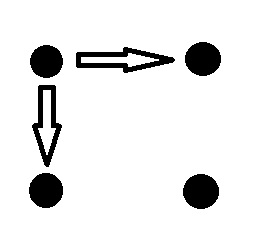
\includegraphics[width=0.5\textwidth]{22lattice}
\caption{A two by two lattice and how they interact using the Ising model}
\label{fig:22lattice}
\end{figure}




\newpage

\begin{center}
{\LARGE\bf Method}
\end{center}

\noindent To be able to start programming, one first needs to find the expressions for the partition function $Z$ with its corresponding energy values $E$, the mean magnetic moment $M$, the specific heat $C_V$ and the susceptibility $X$ as functions of the temperature $T$. All of this using the periodic boundary condition.
\\
The partition function $Z$ is giving by: 


$$
Z = \sum^{M}_{i = 1} e^{-\beta * E_i}
$$ 

\noindent where $\beta$ is the inverse temperature given by $\beta = \frac{1}{kT}$ where k is the Boltzmann constant and T is the temperature, so every expression containing $\beta$ is dependent on the temperature $T$. $E_i$ is the energy for different spin settings given by:

$$
E = -J\sum^{N}_{<kl>} s_ks_l
$$

\noindent where J is the coupling constant and N is the total number of spins. $s_k$ and $s_l$ are the spins of two neighbouring objects in a lattice. Since we are working 2x2 lattice, the total number of combinations are given by $2^4 = 16$, considering we are working with the Ising model where the spins can only be $-1$ or $1$.
\\
From \figref{22lattice} we see how the Ising model works on a 2x2 lattice and from this the energy is calculated. One can observe that energy is non-zero on lattices where all the objects have the same spin ($-8J$) and where the two diagonals have opposite spin from each other ($8J$). All other settings have zero energy. Knowing the energy values we can calculate the mean energy $<E>$ with our specific partition function:

$$
<E> = \frac{1}{Z}\sum^{M}_{i = 1} E_i e^{-\beta E_i}
$$
$$
 = \frac{1}{2e^{-8} + 2e^{8} + 12}\sum^{16}_{1} E_i e^{-\beta E_i}
$$
$$
 = \frac{16e^{-8}-16e^{8}}{2e^{-8} + 2e^{8} + 12} = -7.983928
$$

\noindent Now we can simply put the same energy values into our partition function:

$$
Z = e^{-\beta * -8J} + e^{-\beta * -8J} + e^{-\beta * 8J} + e^{-\beta * 8J} + 12*e^0
$$
$$
Z = 2e^{-8J\beta} + 2e^{8J\beta} + 12
$$

\noindent The magnetization is given by:

$$
M = \sum^{N}_{j = 1} s_j
$$

\noindent Unlike in the energy case, the magnetization does not depend the lattice having the same spin or that the diagonals have opposite spin. The only case where the magnetization is zero in a 2x2 lattice is when half of the objects in the lattice opposite spins. Therefore we get the magnetization values:

$$
M_i = [4 + 2 + 2 + 2 + 2 + 0 + 0 + 0 + 0 + 0 + 0 + -2 + -2 + -2 + -2 + -4]
$$

\noindent To calculate the mean magnetic moment or mean magnetization we use the equation below with our calculated magnetic moment and energy values:

$$
|M| = \frac{1}{Z}\sum^{M}_{i}M_ie^{-\beta E_i}
$$
$$
 = \frac{1}{2e^{-8} + 2e^8 + 12}\sum^{16}_{1}M_ie^{-\beta E_i}
$$
$$
 = \frac{8e^{8} + 16}{2e^{-8} + 2e^8 + 12} = 3.994643
$$



\noindent To calculate the the specific heat, one only needs to know the total number of spins of the lattice. In the 2x2 lattice case the total number of spins is 4, and remember also that $\beta J = 1$ and $k = 1$. The specific heat is then:

$$
C_V = \frac{1}{kT^2}(<E^2> - <E>^2)
$$
$$
 = \frac{1}{kT^2}(\frac{128e^{-8} - 128e^8}{2e^{-8} + 2e^8 + 12} - (\frac{16e^{-8} - 16e^8}{2e^{-8} + 2e^8 + 12})^2)
$$
$$
 = 0.128329
$$

\noindent The term $<E^2> - <E>^2$ is also called the variance of the energy and is precisely calculated just as shown above. The same variance calculation can be applied to calculating the susceptibility, but the energy terms have to be substituted for mean magnetization.
Let's calculate the variance separate from the desired equation this time:

$$
\sigma_M^2 = <M^2>-<M>^2 = \frac{1}{Z}\sum^{M}_{i = 1}M_i^2 e^{-\beta E_i} - (\frac{1}{Z}\sum^{M}_{i = 1}M_i e^{-\beta E_i})^2
$$

$$
 = \frac{32}{2e^{-8} + 2e^8 + 12}(e^{8}+1) - (\frac{8e^8 + 16}{2e^{-8} + 2e^8 + 12})^2 = 0.016004
$$

\noindent Remember that the $\beta = 1$ in the 2x2 lattice case, so the susceptibility would be the same as the variance in that case. We would usually have to calculate the susceptibility with the following equation:

$$
X = \frac{1}{k_bT}(<M^2> - <M>^2) = \frac{1}{k_bT}\sigma_M^2 = 0.010853
$$

\noindent To compute the above values, a standard Metropolis algorithm were implemented (kilde). This algorithm takes in a matrix, only ones or negative ones in this case, and then decides to flip or not flip the current value at a random location in the matrix (lattice). The probability of when to flip or not is in this case given by the Boltzmann distribution $e^{-E_i / T}$. If the algorithm decides to flip, the computed energy at that position in the lattice is added to the total energy of the system. The same happens for the magnetization. Initial values of the energy and magnetization is calculated beforehand. What initial matrix to use, that is a randomly generated matrix or a matrix with only positive spin, is determined by the user. After the Metropolis algorithm is finished, the cumulative energy, squared cumulative energy, cumulative magnetization and cumulative magnetization squared is calculated which is needed to later calculate the mean energy, mean magnetization, specific heat and susceptibility. This algorithm is based on random events and so one needs to perform the algorithm many times before the results are stable. Therefore the whole Metropolis algorithm is looped inside what is called a Monte Carlo loop. When the number of cycles are increased, the more stable the results will be. However, many cycles require a lot of processing power when the number of cycles get to around $10^6$.
\\
To be able to run the program in a time efficient manner, one needs to parallellize the program, and this was done by using MPI with 8 processors. Using MPI made the processing time much smaller, but it still took a long time for large lattice sizes.
\\
Raw data were produced using c++ while plotting and further calculations were done using MatLab. Further calculations include finding the probability distribution and the thermodynamic limit.  
\\
To calculate the critical temperature one have to use the following equation:

$$
T_c(L) - T_c(L=\infty) = aL^{-1/v}
$$

\noindent where $T_c$ is the critical temperature, L is the size of the lattice, $v = 1$ and a is a constant. $T_c(L)$ is known and we then get the following equations which can be solved numerically:

$$
T_c(L) = T_c(L = \infty) + aL^{-1}
$$

\noindent To solve this numerically, one simply have to solve the above equations for both $T_c(L = \infty)$ and $a$. Again, $T_c$ and $L$ is known. The equations were solved in MatLab using the least square rule as the linear regression. By doing this, the values for $T_c(L = \infty)$ and $a$ were found.

\newpage

\begin{center}
{\LARGE\bf Results}
\end{center}

\noindent The specific analytical value found in the method is compared to the numerical value calculated in c++ in the table below:

\begin{table} [H]
\caption{Analytical and numerical solutions} \label{tab:table1}
\centerline{
\begin{tabular}{|c|c|c|c|}
\hline
Type & Analytical & Numerical & MC cycles needed\\
\hline
$<E>$ & -7.983928 & -7.98437 & 10 000\\
\hline
$<M>$ & 3.994643 & 3.99483 & 10 000\\
\hline
$C_V$ & 0.128329 & 0.124812 & 100 000\\
\hline
$<X>$ & 0.016004 & 0.0153613 & 100 000\\
\hline
\end{tabular}
}
\end{table}

\noindent To get good results for mean energy and mean magnetization took very few Monte Carlo cycles, only about $10^4$. Then the values would be off only by a factor of about $10^{-3}$. The susceptibility and the specific heat took more Monte Carlo cycles to get a precise and stable result. Correct results started showing around $10^{5}$. For $10^4$, both the specific heat and susceptibility gave unstable results. 
\\
The values shown in Table \ref{tab:table1} are representing each object in the lattice, but for the rest of the paper the values will be calculated for the entirety of the lattice. To transition from lattice wide values to single object values, one simply have to divide by the size of the lattice, $4$ in the above case, and multiply in the reverse case.

\begin{figure}[H]
\centerline{
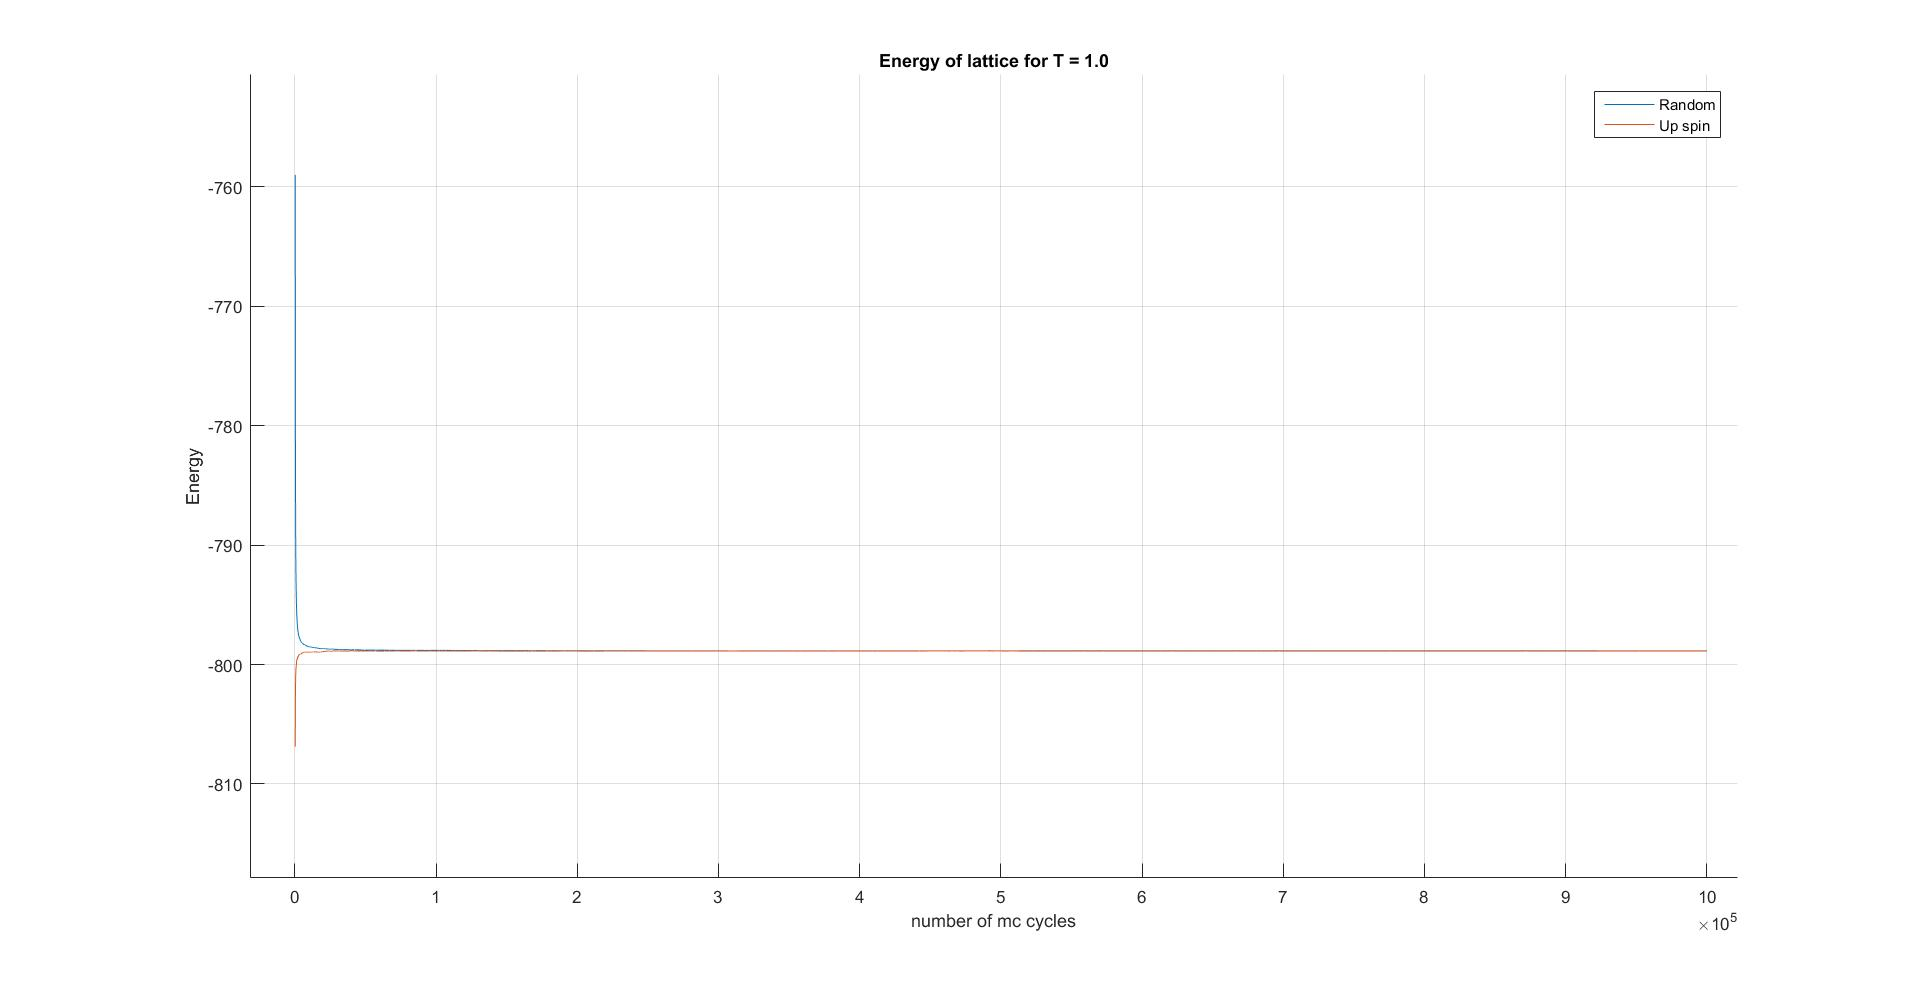
\includegraphics[width=0.7\textwidth]{energy1T}
}
\caption{Energy versus Monte Carlo cycles for T = 1.0}
\label{fig:energy1T}
\end{figure}

\begin{figure}[H]
\centerline{
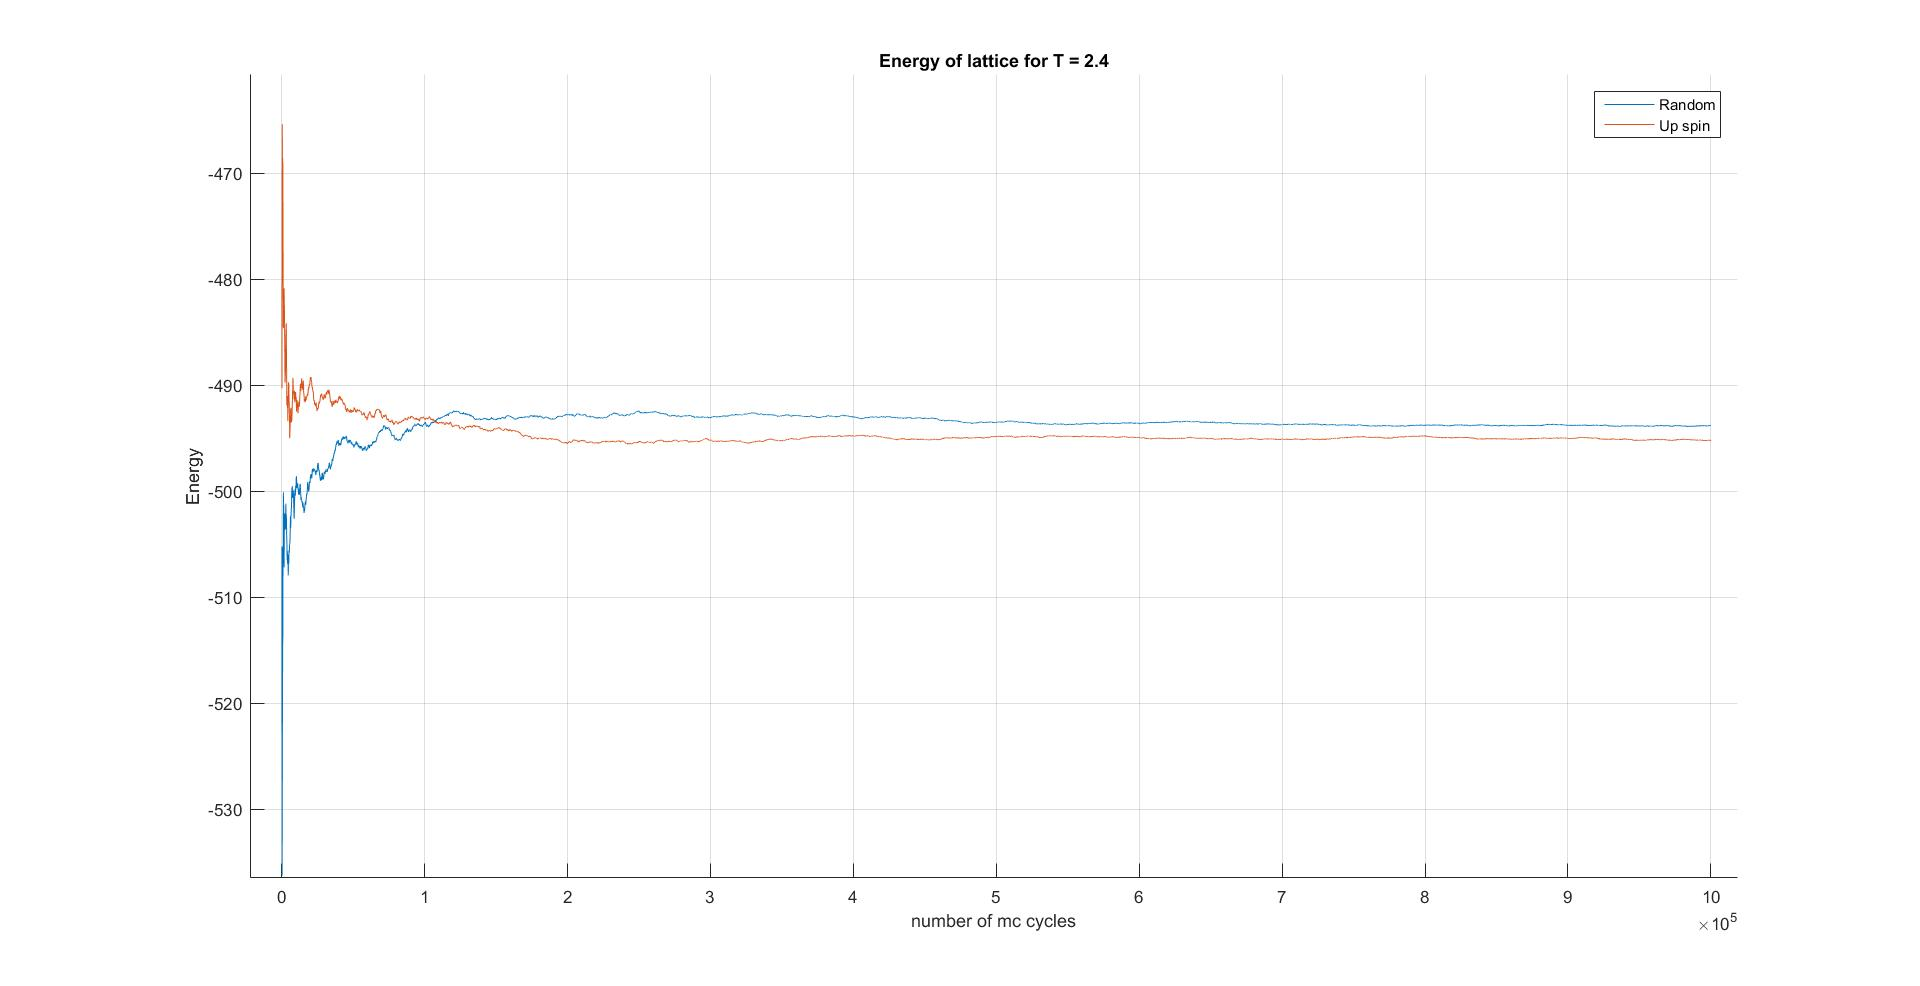
\includegraphics[width=0.7\textwidth]{energy24T}
}
\caption{Energy versus Monte Carlo cycles for T = 2.4}
\label{fig:energy24T}
\end{figure}

\begin{figure}[H]
\centerline{
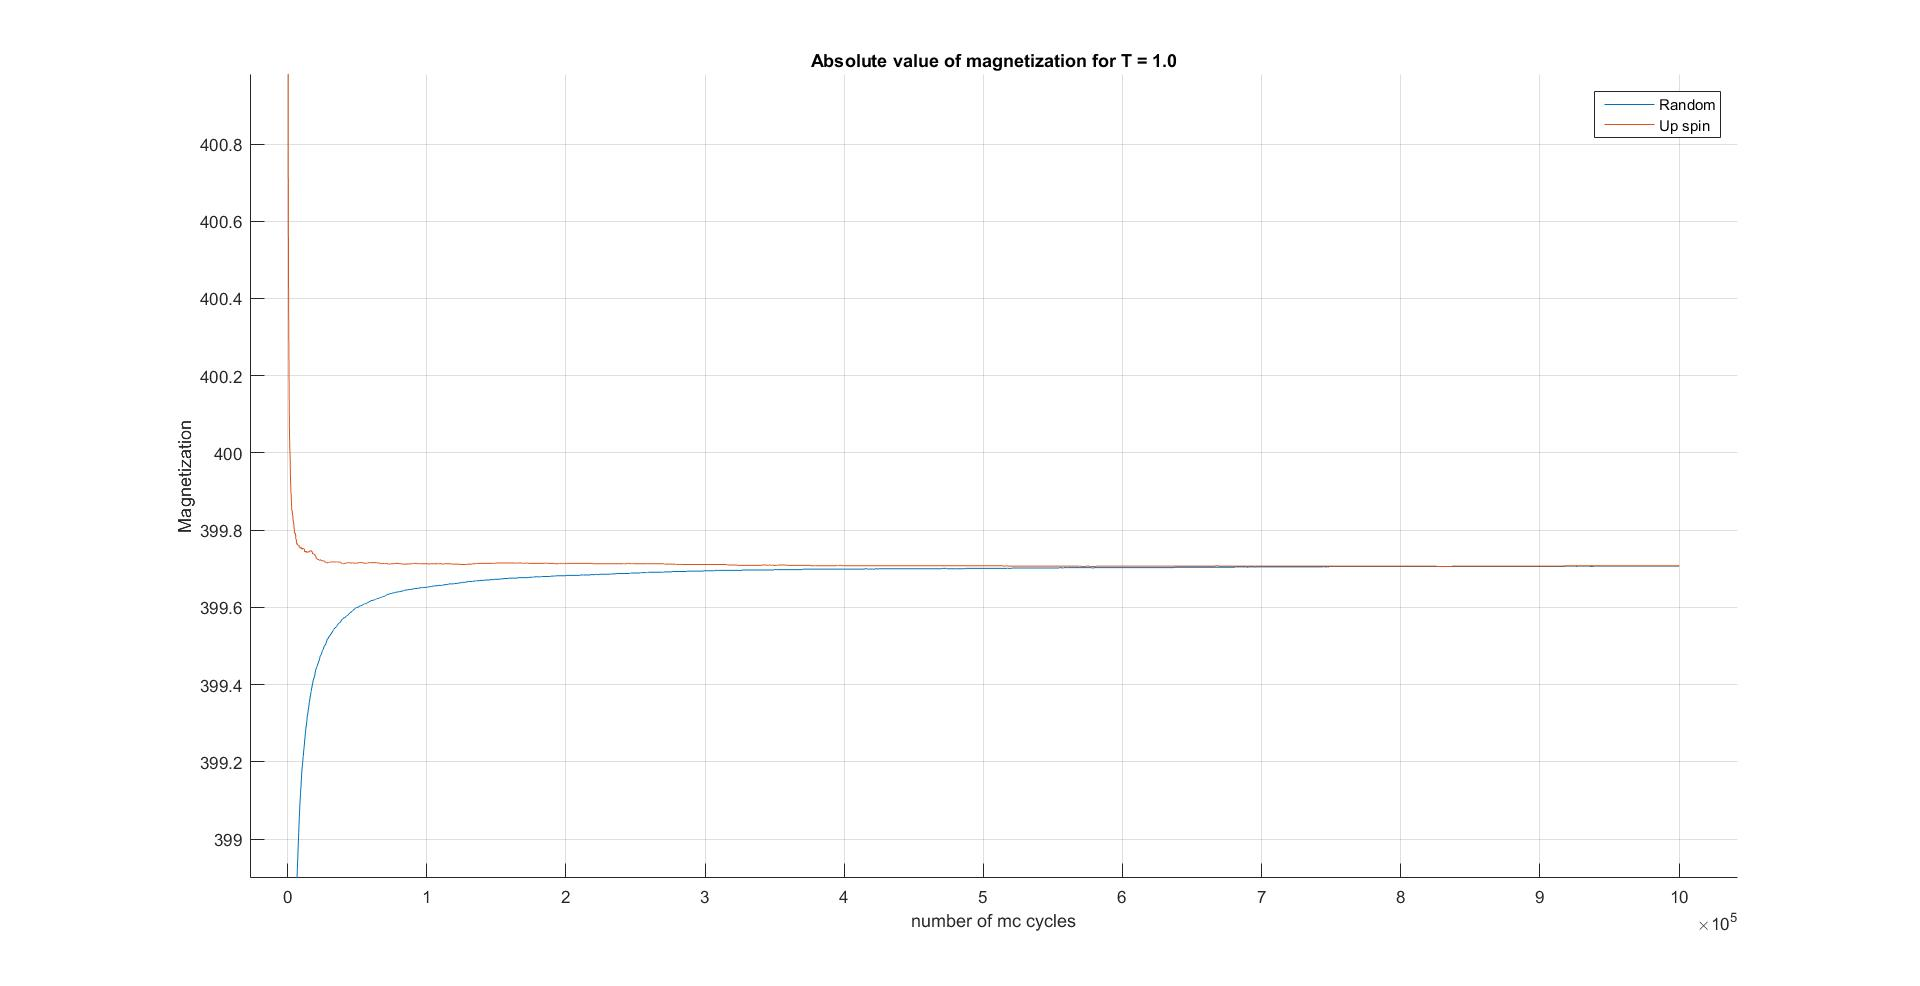
\includegraphics[width=0.7\textwidth]{absmag1T}
}
\caption{Absolute value of magnetization versus Monte Carlo cycles for T = 1.0}
\label{fig:absmag1T}
\end{figure}

\begin{figure}[H]
\centerline{
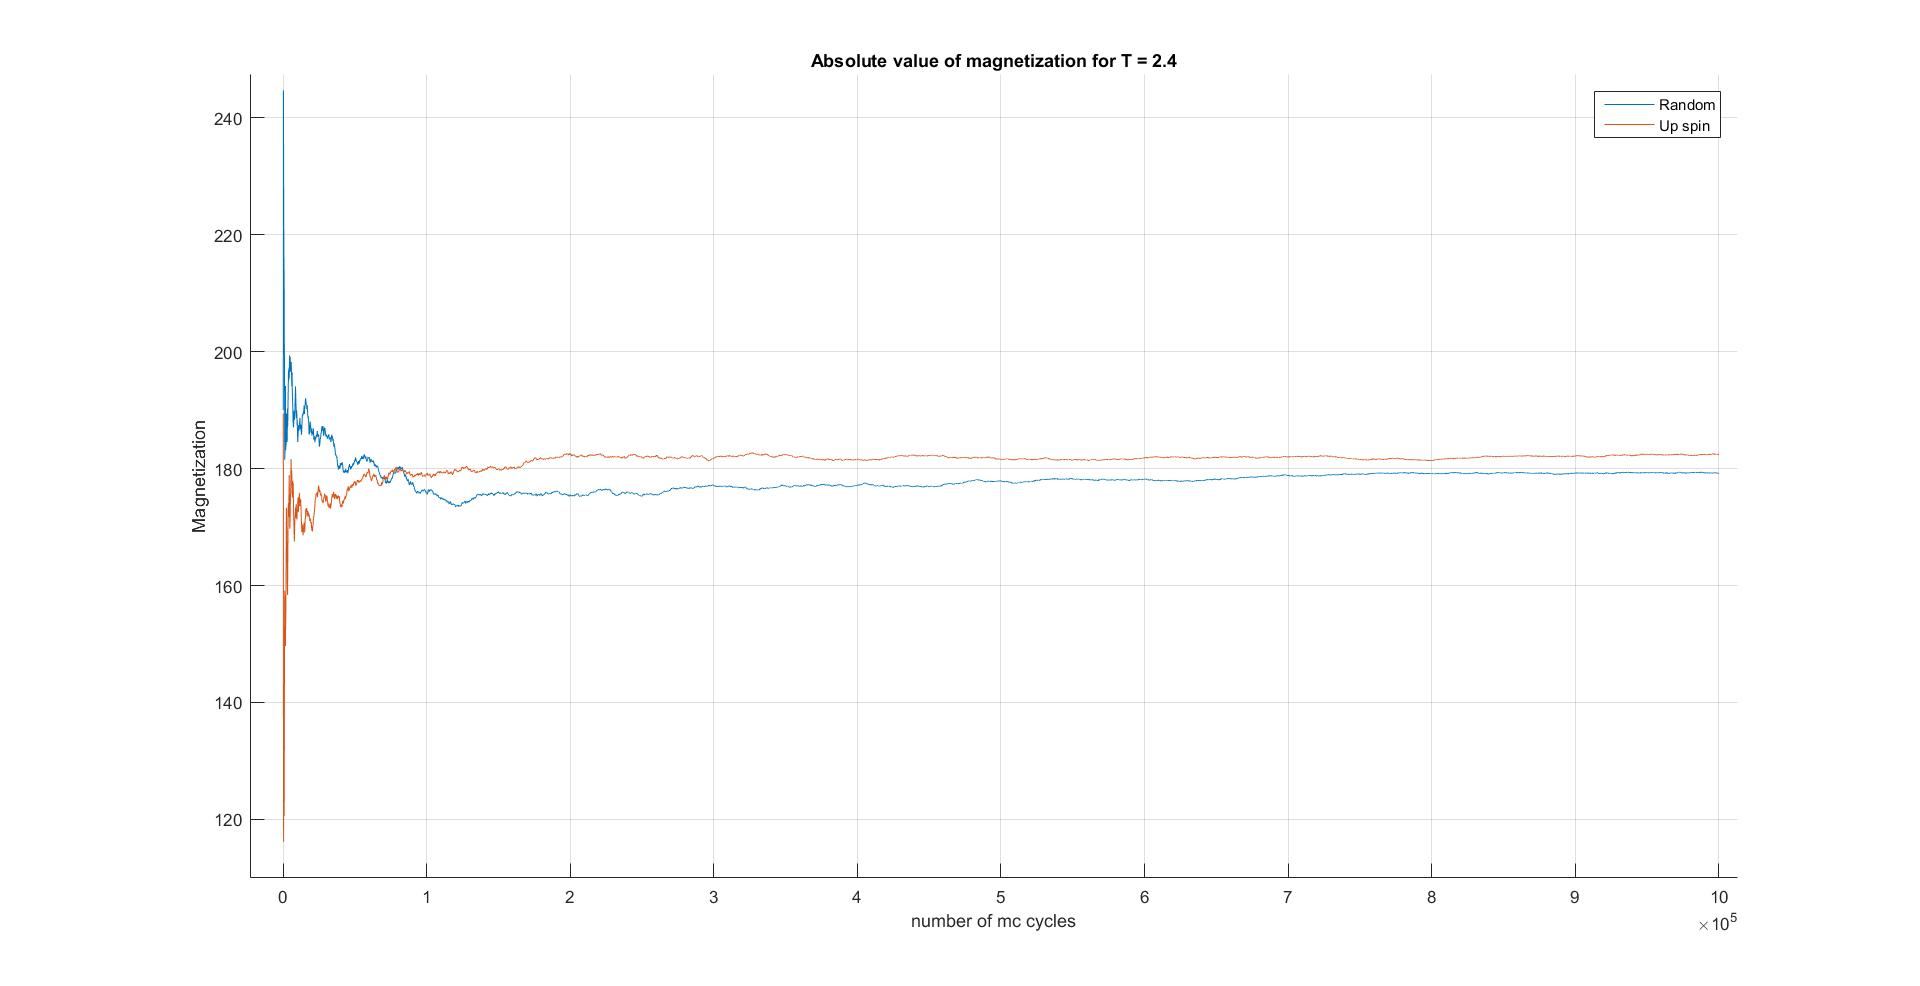
\includegraphics[width=0.7\textwidth]{absmag24T}
}
\caption{Absolute value of magnetization versus Monte Carlo cycles for T = 2.4}
\label{fig:absmag24T}
\end{figure}
\begin{figure}[H]
\centerline{
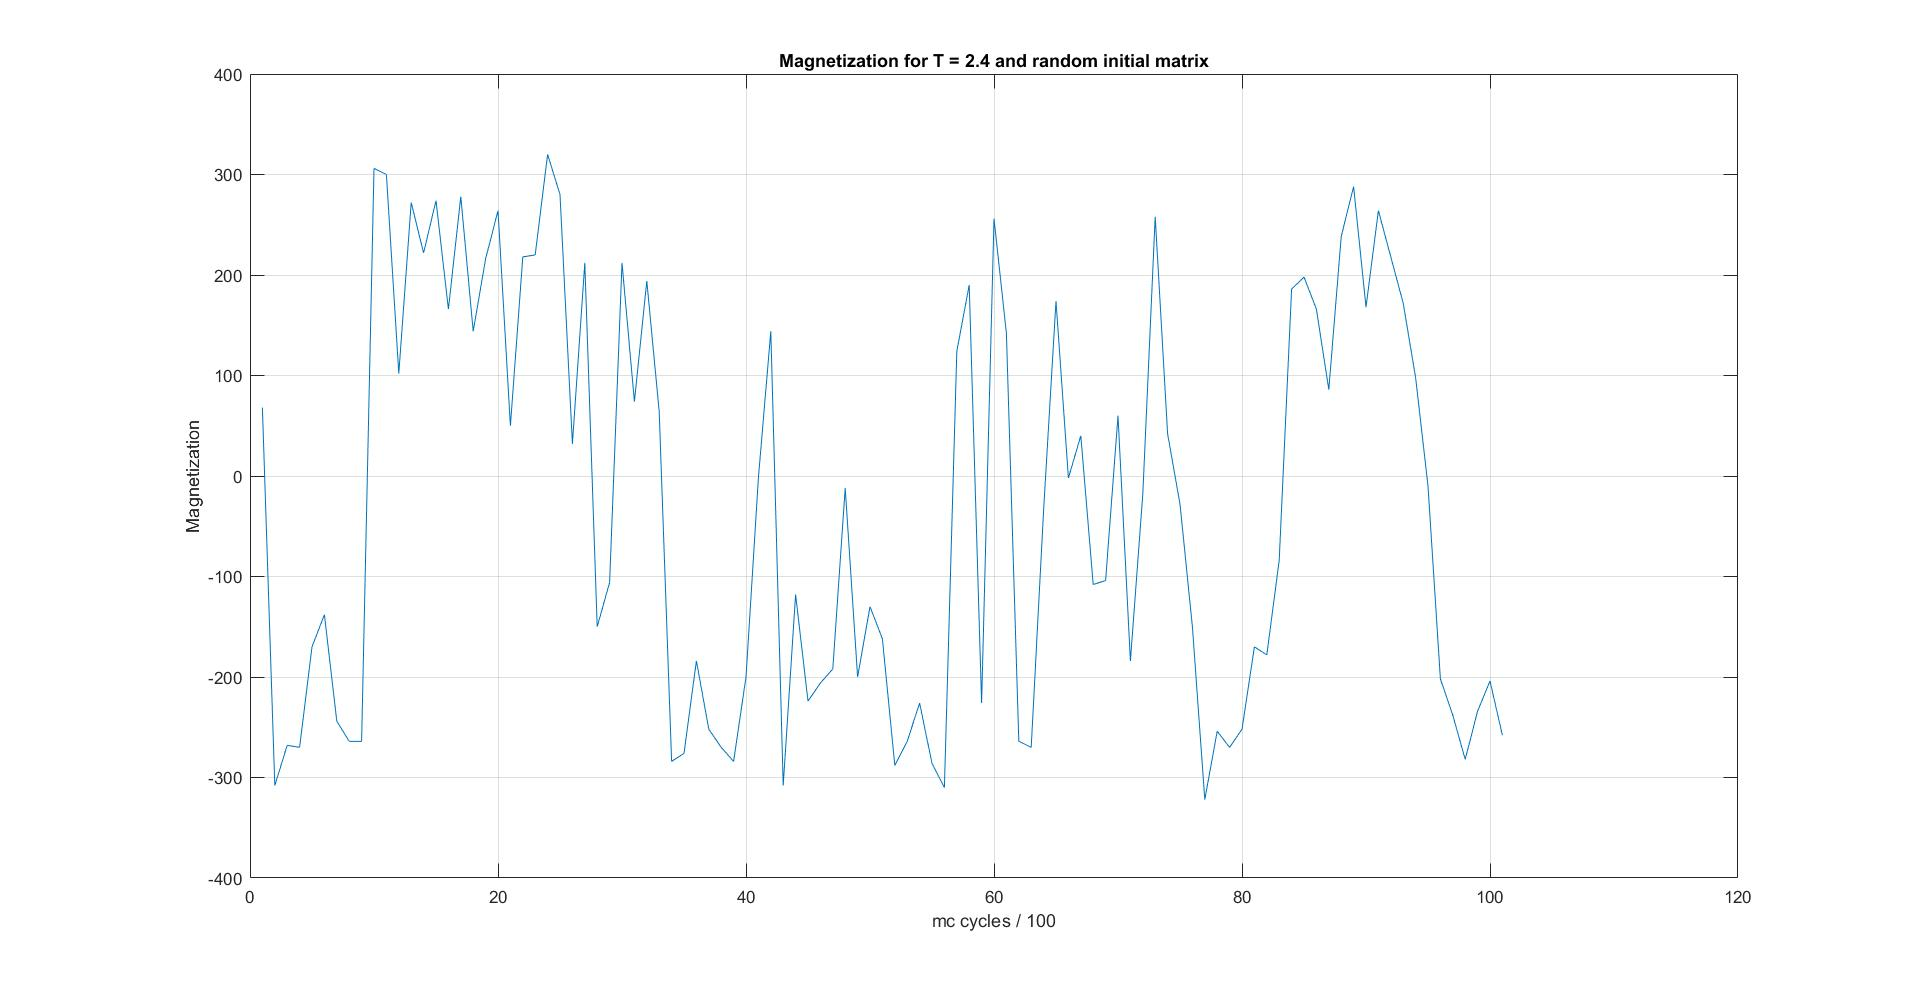
\includegraphics[width=0.7\textwidth]{magnetizationT24random}
}
\caption{Mean magnetization versus Monte Carlo cycles for T = 2.4}
\label{fig:mag24T}
\end{figure}
\begin{figure}[H]
\centerline{
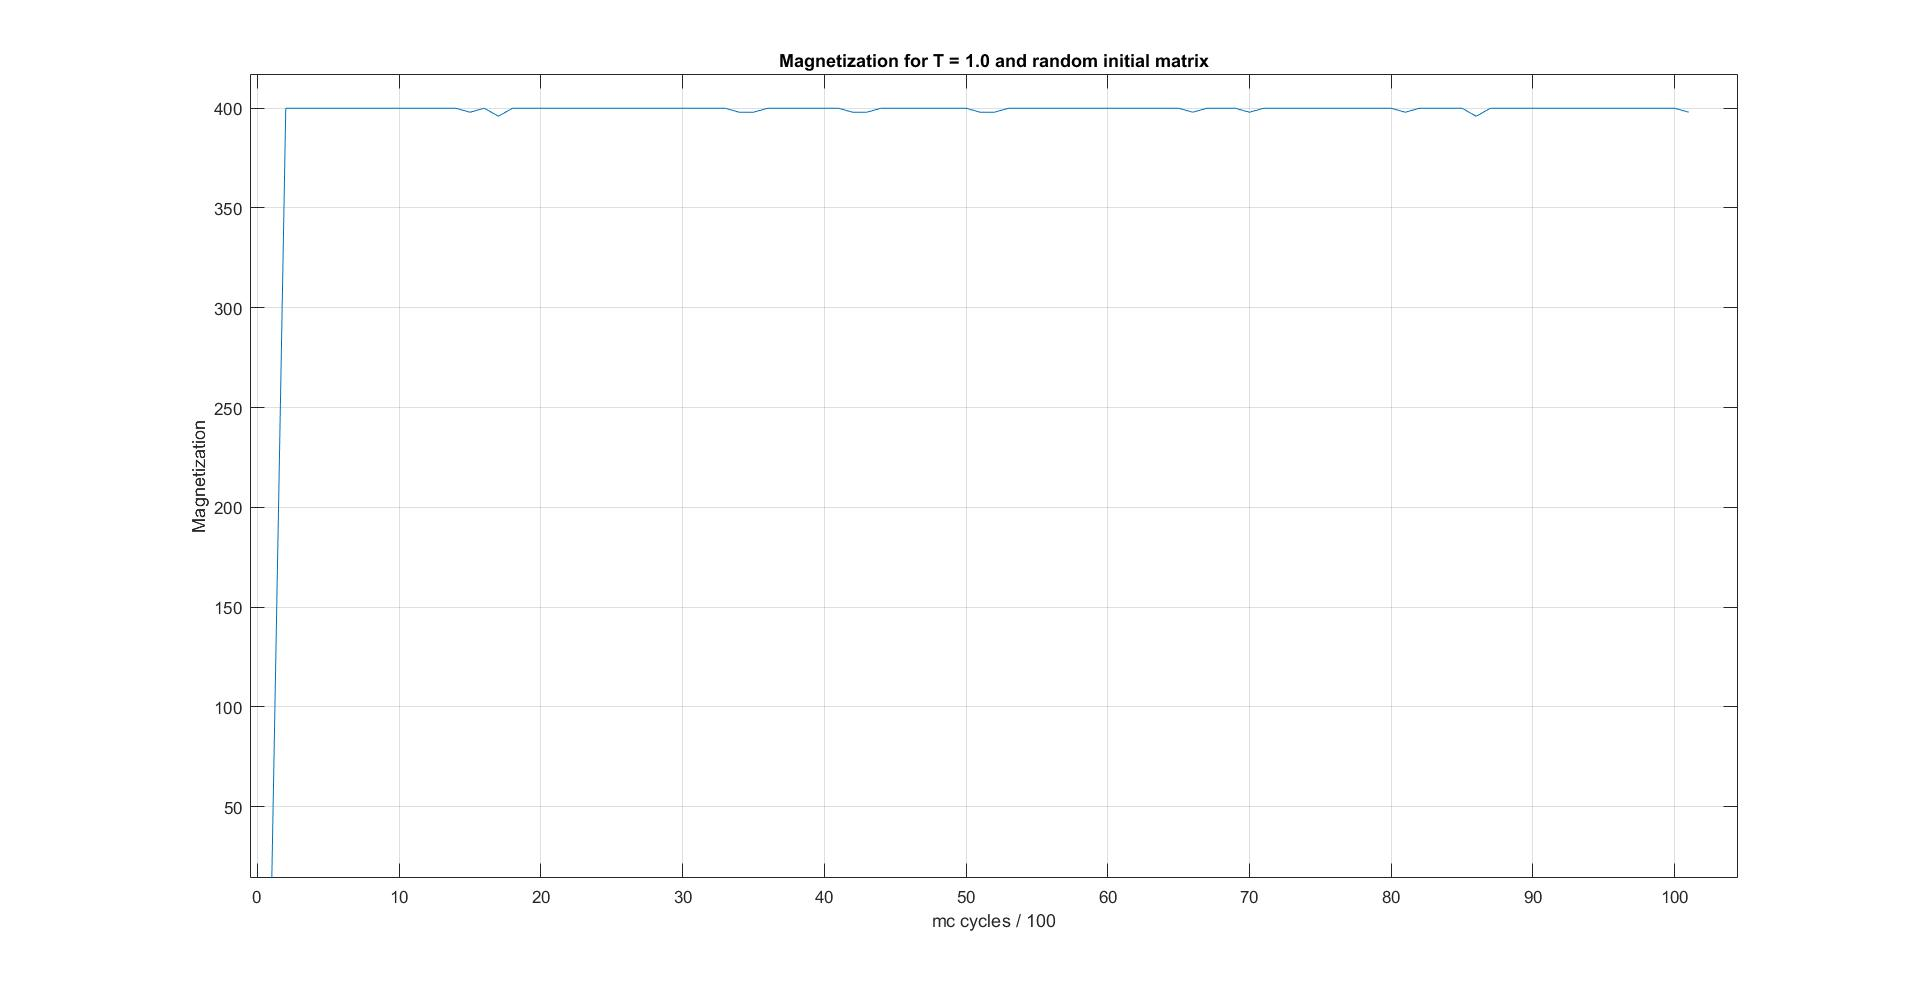
\includegraphics[width=0.7\textwidth]{magnetizationT1random}
}
\caption{Mean magnetization versus Monte Carlo cycles for T = 1.0}
\label{fig:mag1T}
\end{figure}

\noindent One can see from \figref{energy1T}, \figref{energy24T}, \figref{absmag1T} and \figref{absmag24T} that the mean energy and magnetization approaches it's equilibrium state. There are fluctuations after the mean energy and magnetization has reached it's equilibrium state, but the value seems to jump back to to the equilibrium state quickly. The values become more unstable when $T = 2.4$, and also the value of the equilibrium state is changed. The number of Monte Carlo cycles needed to hit equilibrium is different for different temperatures, but the initial matrix that is used do not seem to affect the time it takes to reach equilibrium. The table below gives an approximation of how many Monte Carlo cycles are needed:

\begin{table} [H]
\caption{EQ values for energy} \label{tab:table2}
\centerline{
\begin{tabular}{|c|c|c|c|}
\hline
Orientation & Temperature & EQ state & max MC cycles needed\\
\hline
Random & 1.0 & -790.881 & $2*10^4$\\
\hline
Random & 2.4 & -496.494 & $6*10^5$\\
\hline
Up spin & 1.0 & -798.96 & $2*10^4$\\
\hline
Up spin & 2.4 & -493.996 & $6*10^5$\\
\hline
\end{tabular}
}
\end{table}

\begin{table}[H]
\caption{EQ values for magnetization} \label{tab:table3}
\centerline{
\begin{tabular}{|c|c|c|c|}
\hline
Orientation & Temperature & EQ state & max MC cycles needed\\
\hline
Random & 1.0 & 398.762 & $6*10^5$\\
\hline
Random & 2.4 & 165.209 & $2*10^5$\\
\hline
Up spin & 1.0 & 399.732 & $10^5$\\
\hline
Up spin & 2.4 & 176.087 & $2*10^5$\\
\hline
\end{tabular}
}
\end{table}

\begin{figure}[H]
\centerline{
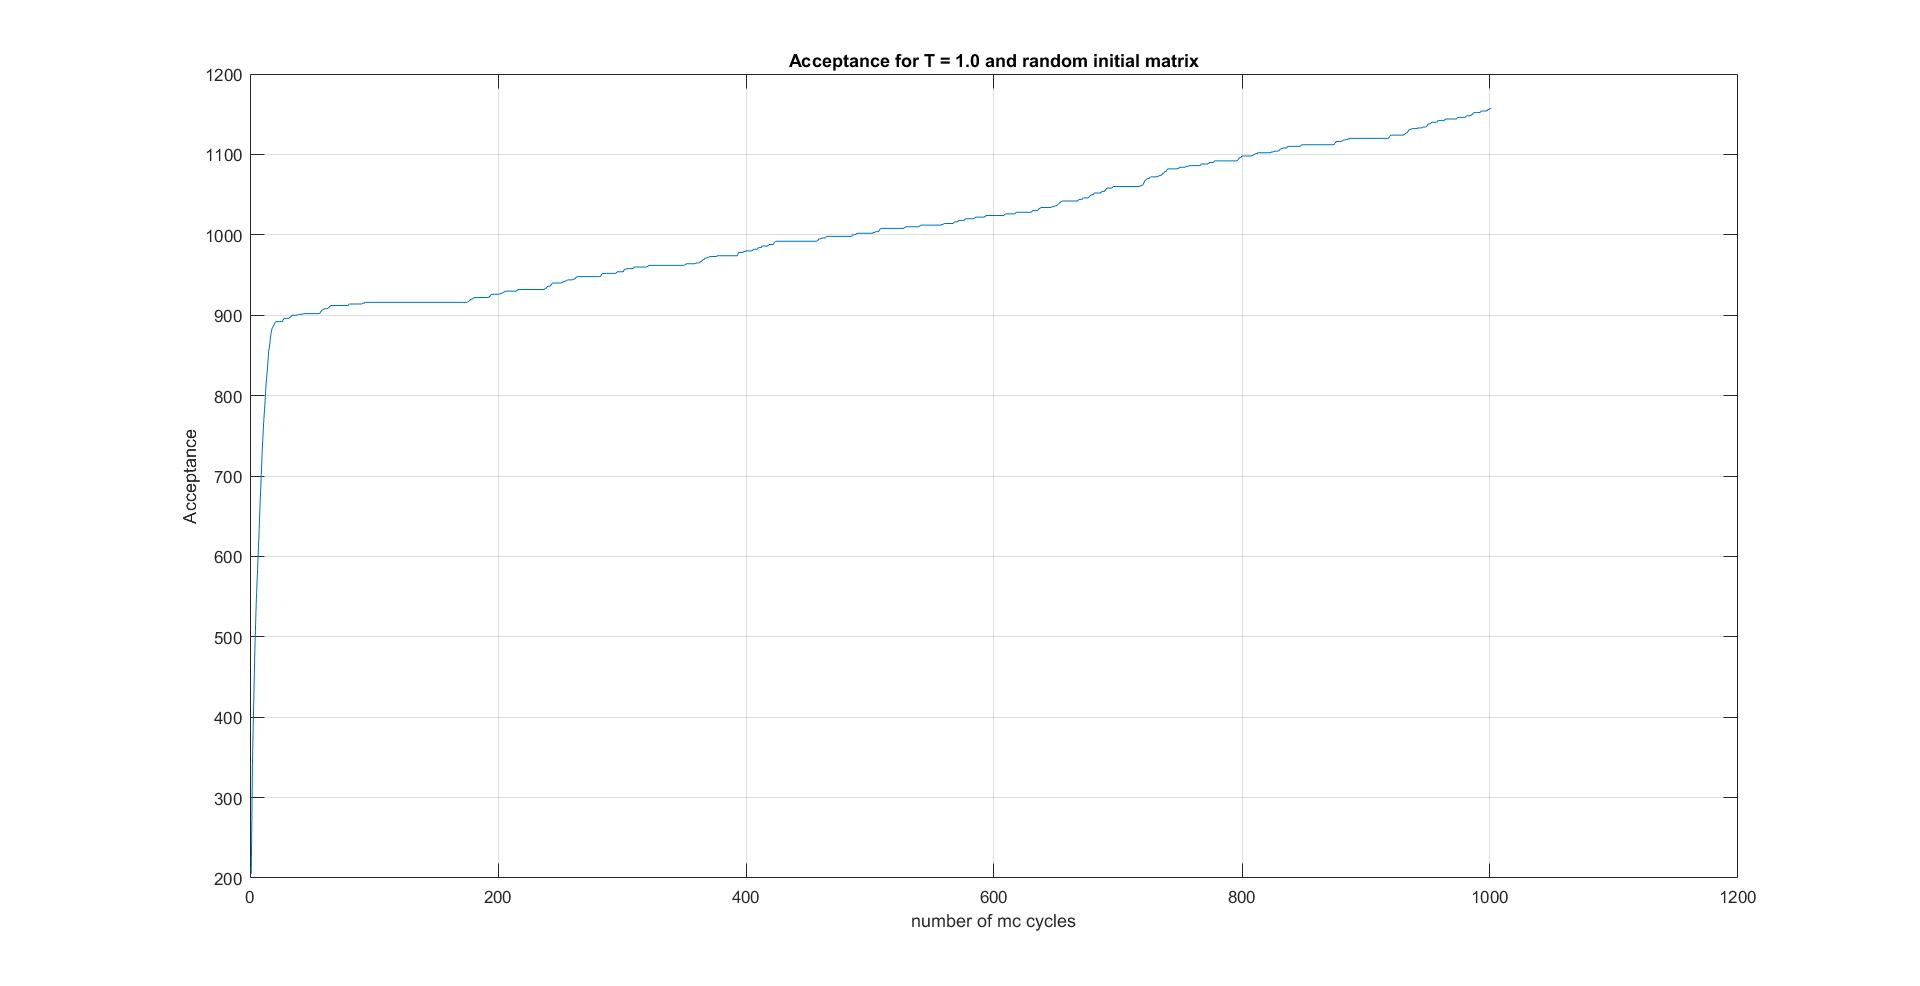
\includegraphics[width=0.7\textwidth]{acceptanceMCT1random}
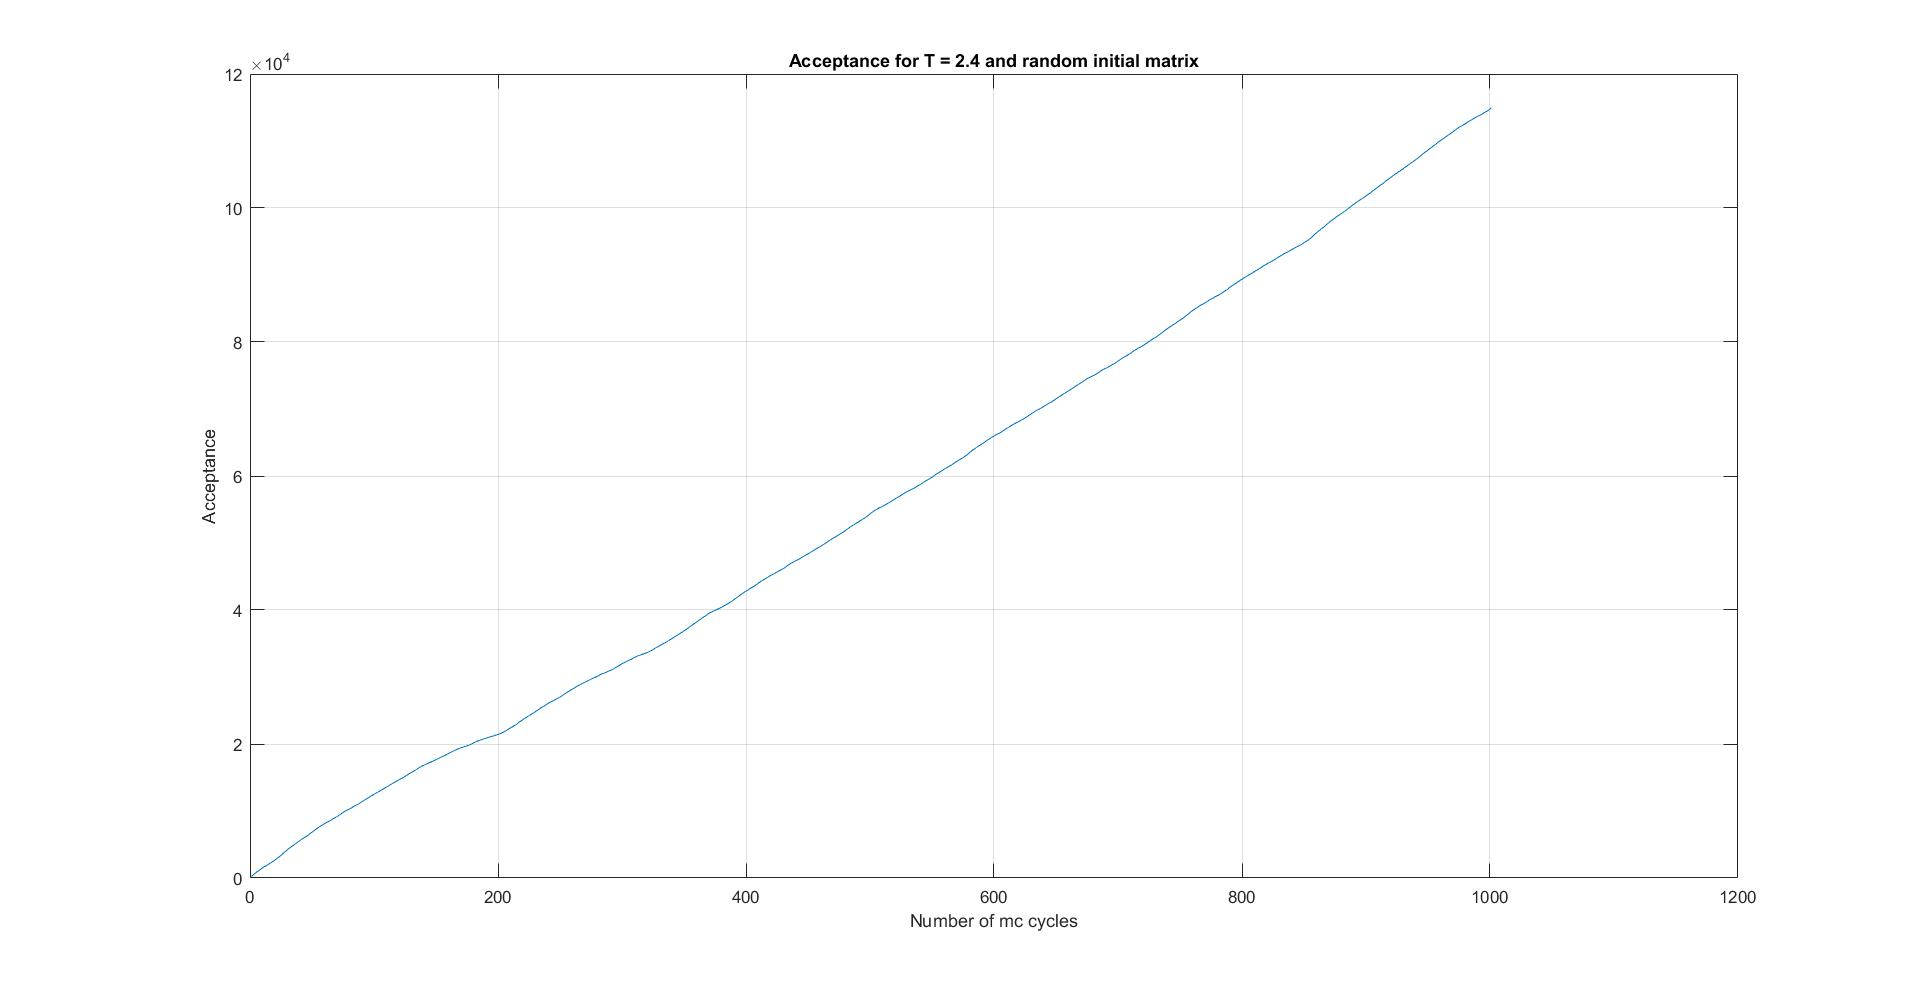
\includegraphics[width=0.7\textwidth]{acceptanceMCT24random}
}
\caption{Acceptance versus Monte Carlo cycles for T = 1.0 and T = 2.4 with a random initial matrix}
\label{fig:acceptancerandom}
\end{figure}

\begin{figure}[H]
\centerline{
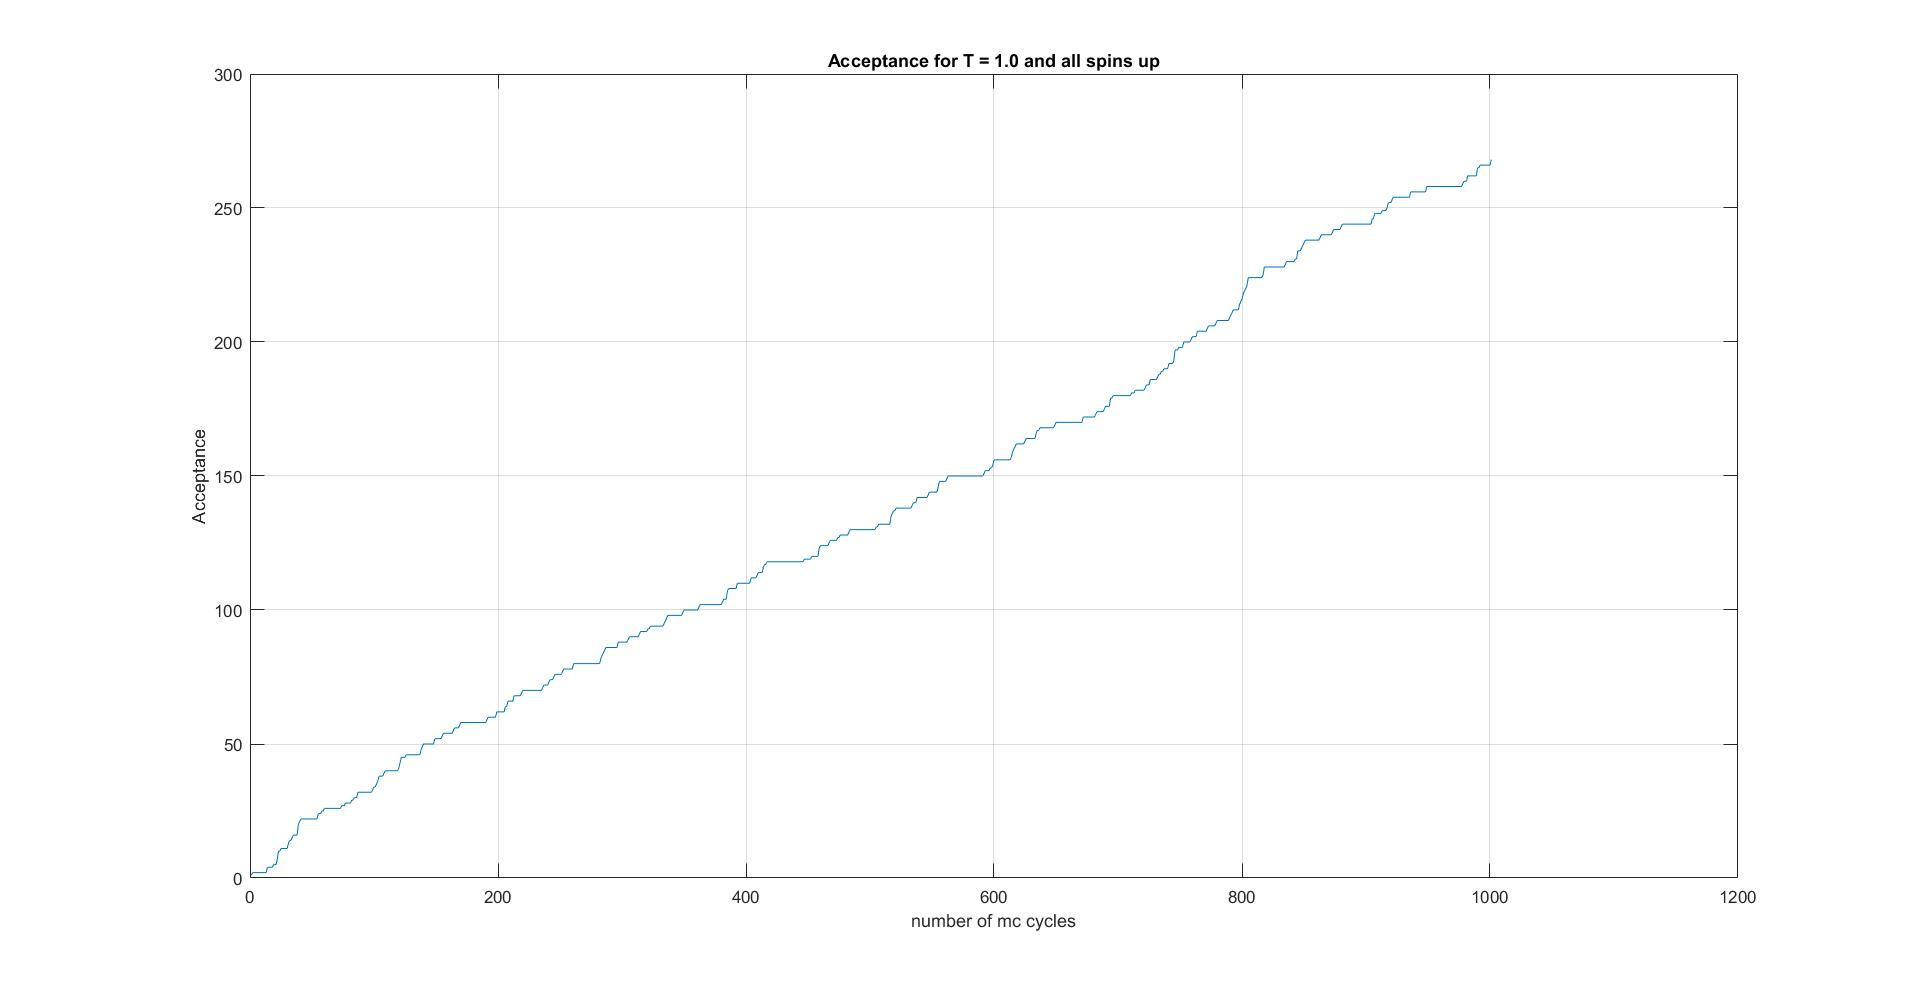
\includegraphics[width=0.7\textwidth]{acceptanceMCT1upspin}
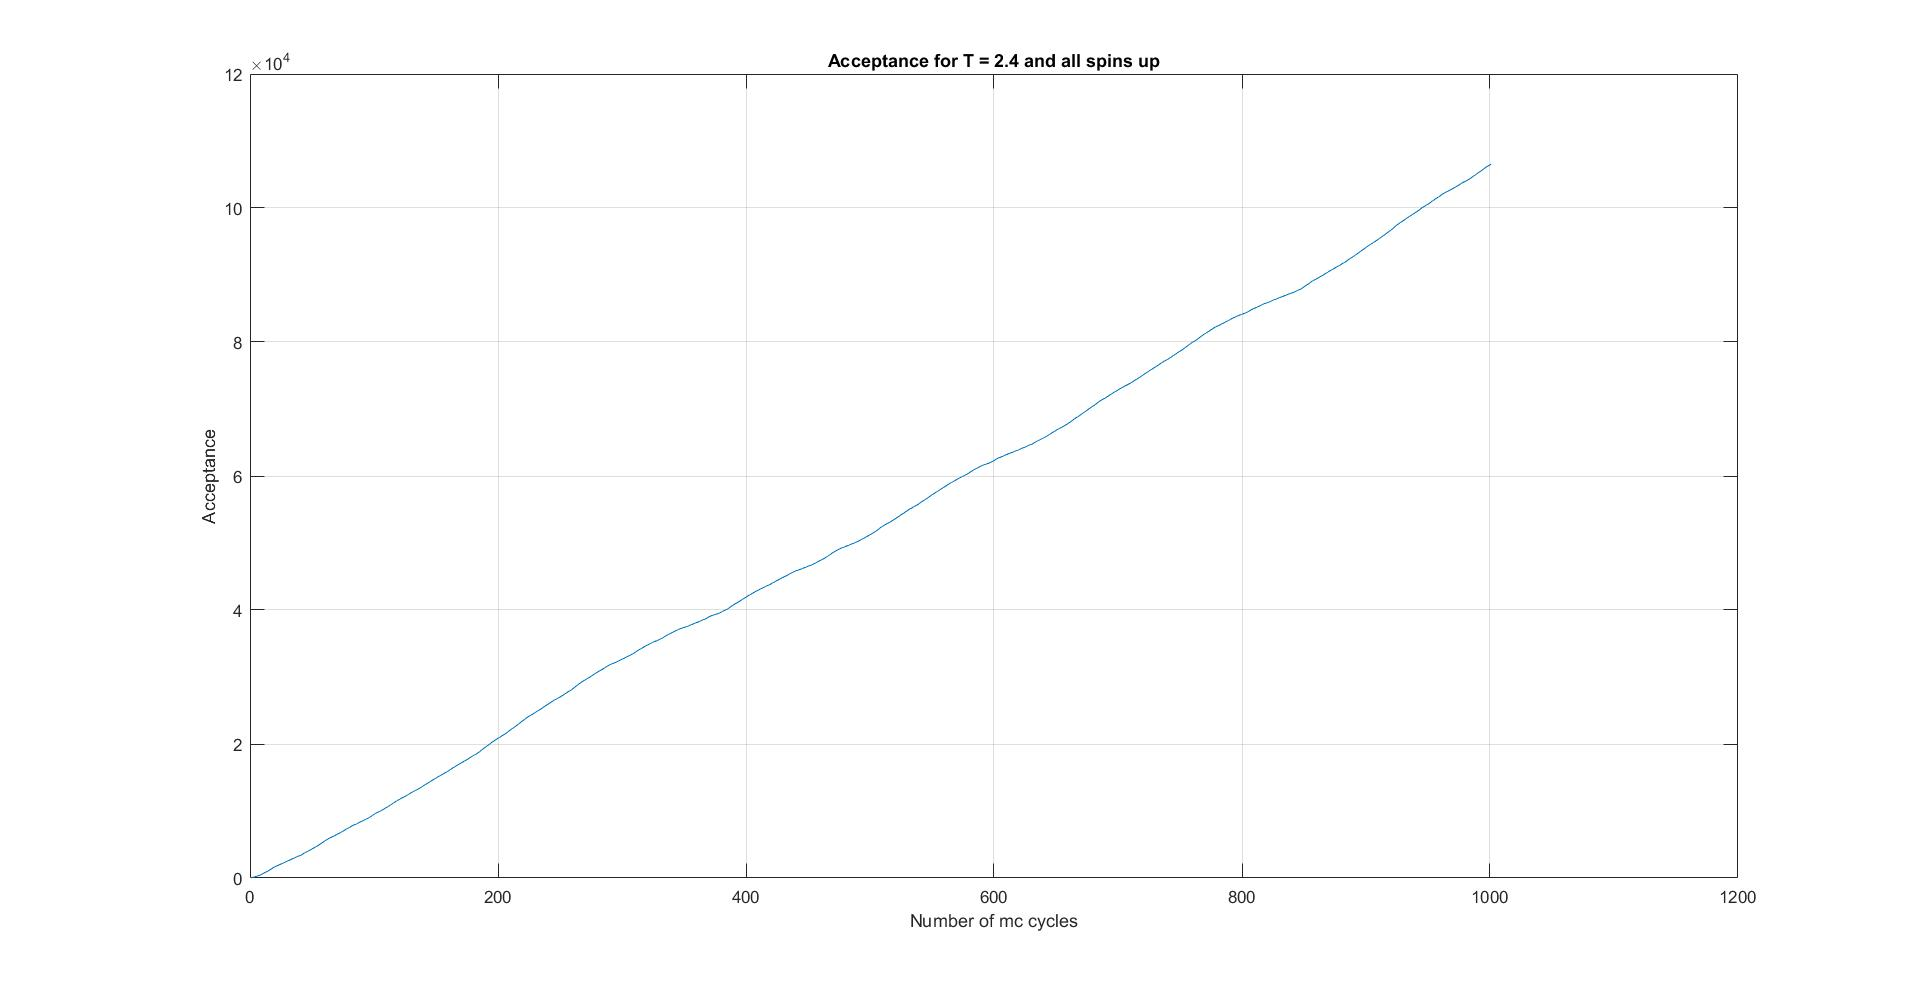
\includegraphics[width=0.7\textwidth]{acceptanceMCT24upspin}
}
\caption{Acceptance versus Monte Carlo cycles for T = 1.0 and T = 2.4 with initial spin upwards}
\label{fig:acceptanceupspin}
\end{figure}

\begin{figure}[H]
\centerline{
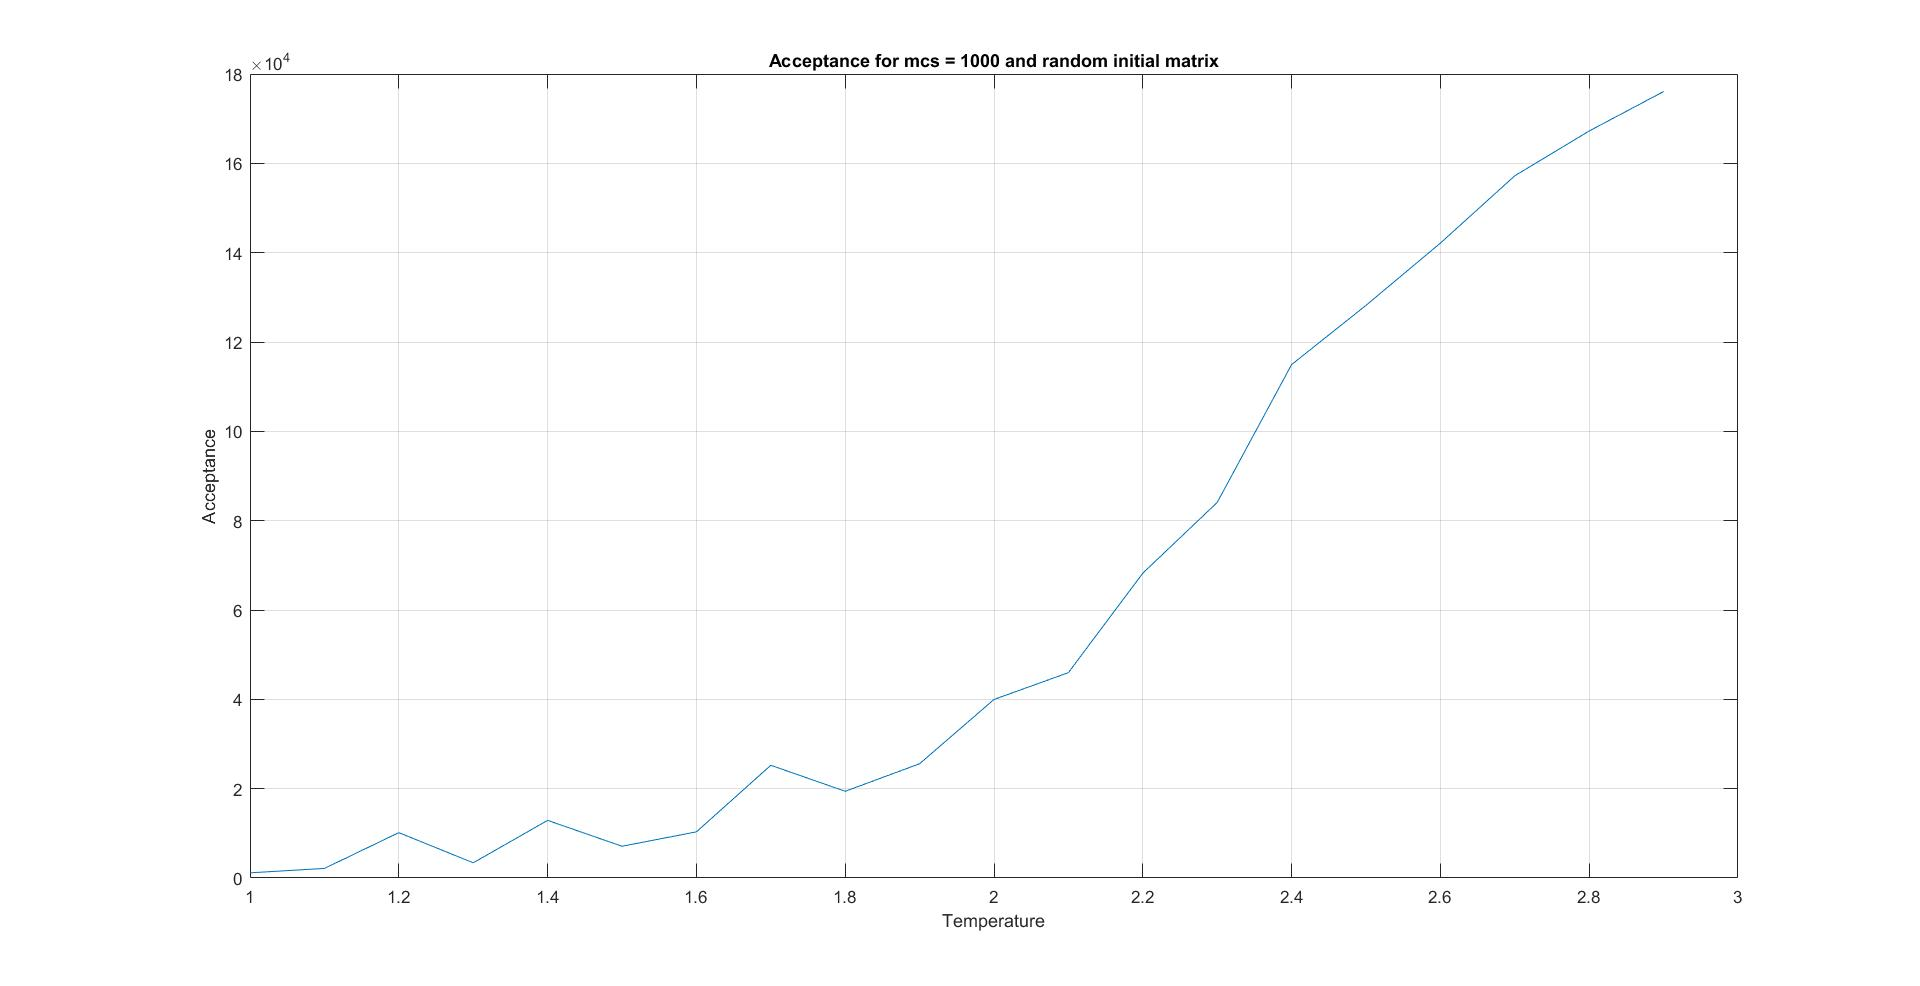
\includegraphics[width=0.7\textwidth]{acceptanceVStrandom}
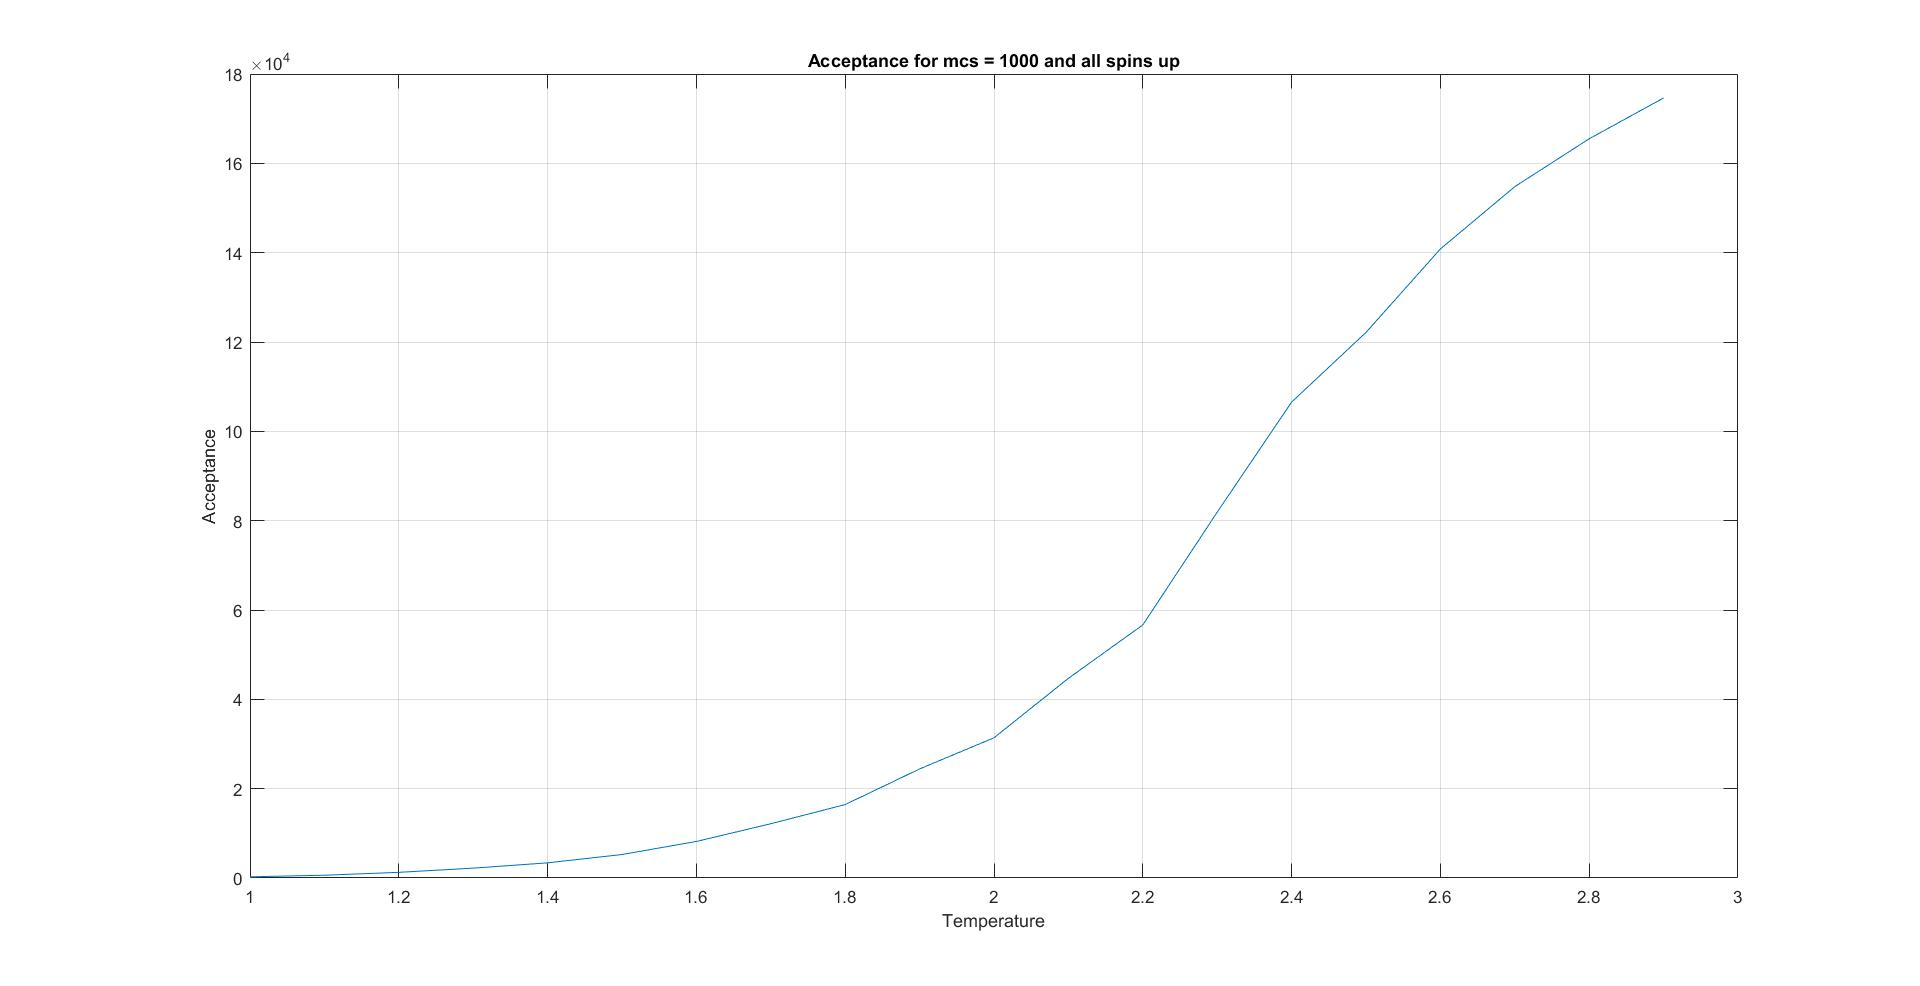
\includegraphics[width=0.7\textwidth]{acceptanceVStupspin}
}
\caption{Acceptance versus temperature for a random initial matrix and with initial spin upwards}
\label{fig:acceptancetemp}
\end{figure}

\noindent Acceptance is apparently dependent on both temperature and the initial state of the spins. From figure \figref{acceptancerandom} one can observe that with higher temperature the number of accepted values increase by a factor of $10$. For $T = 1.0$, one can also observe that the acceptance spikes for few Monte Carlo cycles. 
\\
If the initial spins are all positive like in \figref{acceptanceupspin}, the acceptance becomes more linear. The line for $T = 1.0$ is more squiggly than the straighter line for $T = 2.4$. The ladder does not spike for few Monte Carlo cycles in this case.
\\
From \figref{acceptancetemp}, one can observe that the curves are not linear. The curve based on a randomly generated initial matrix is uneven at low temperatures, but smooths out when $T$ increases. When the initial matrix only consist positive spins, the curve is smooth throughout. These two plots are plotted to a maximum temperature of $3.0$, so one would have an idea of how the acceptance would evolve after $T = 2.4$. 

\begin{figure}[H]
\centerline{
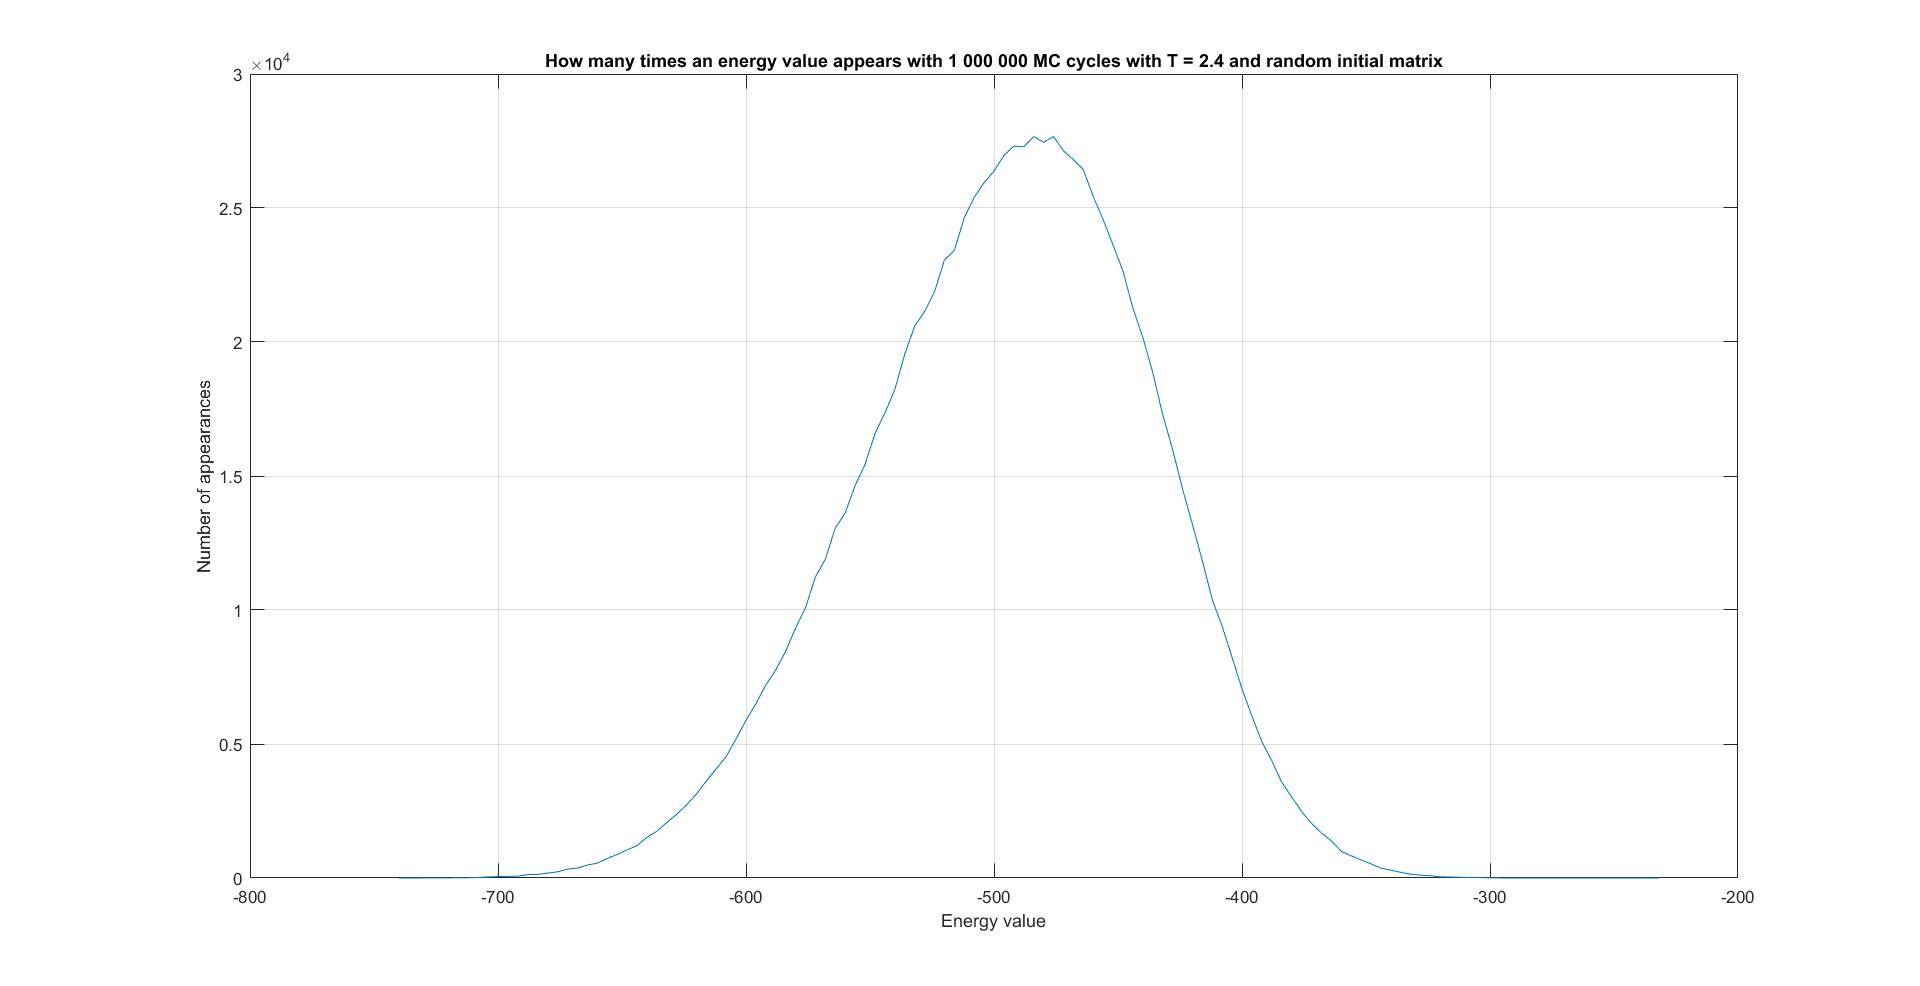
\includegraphics[width=0.7\textwidth]{energyappearanceT24random}
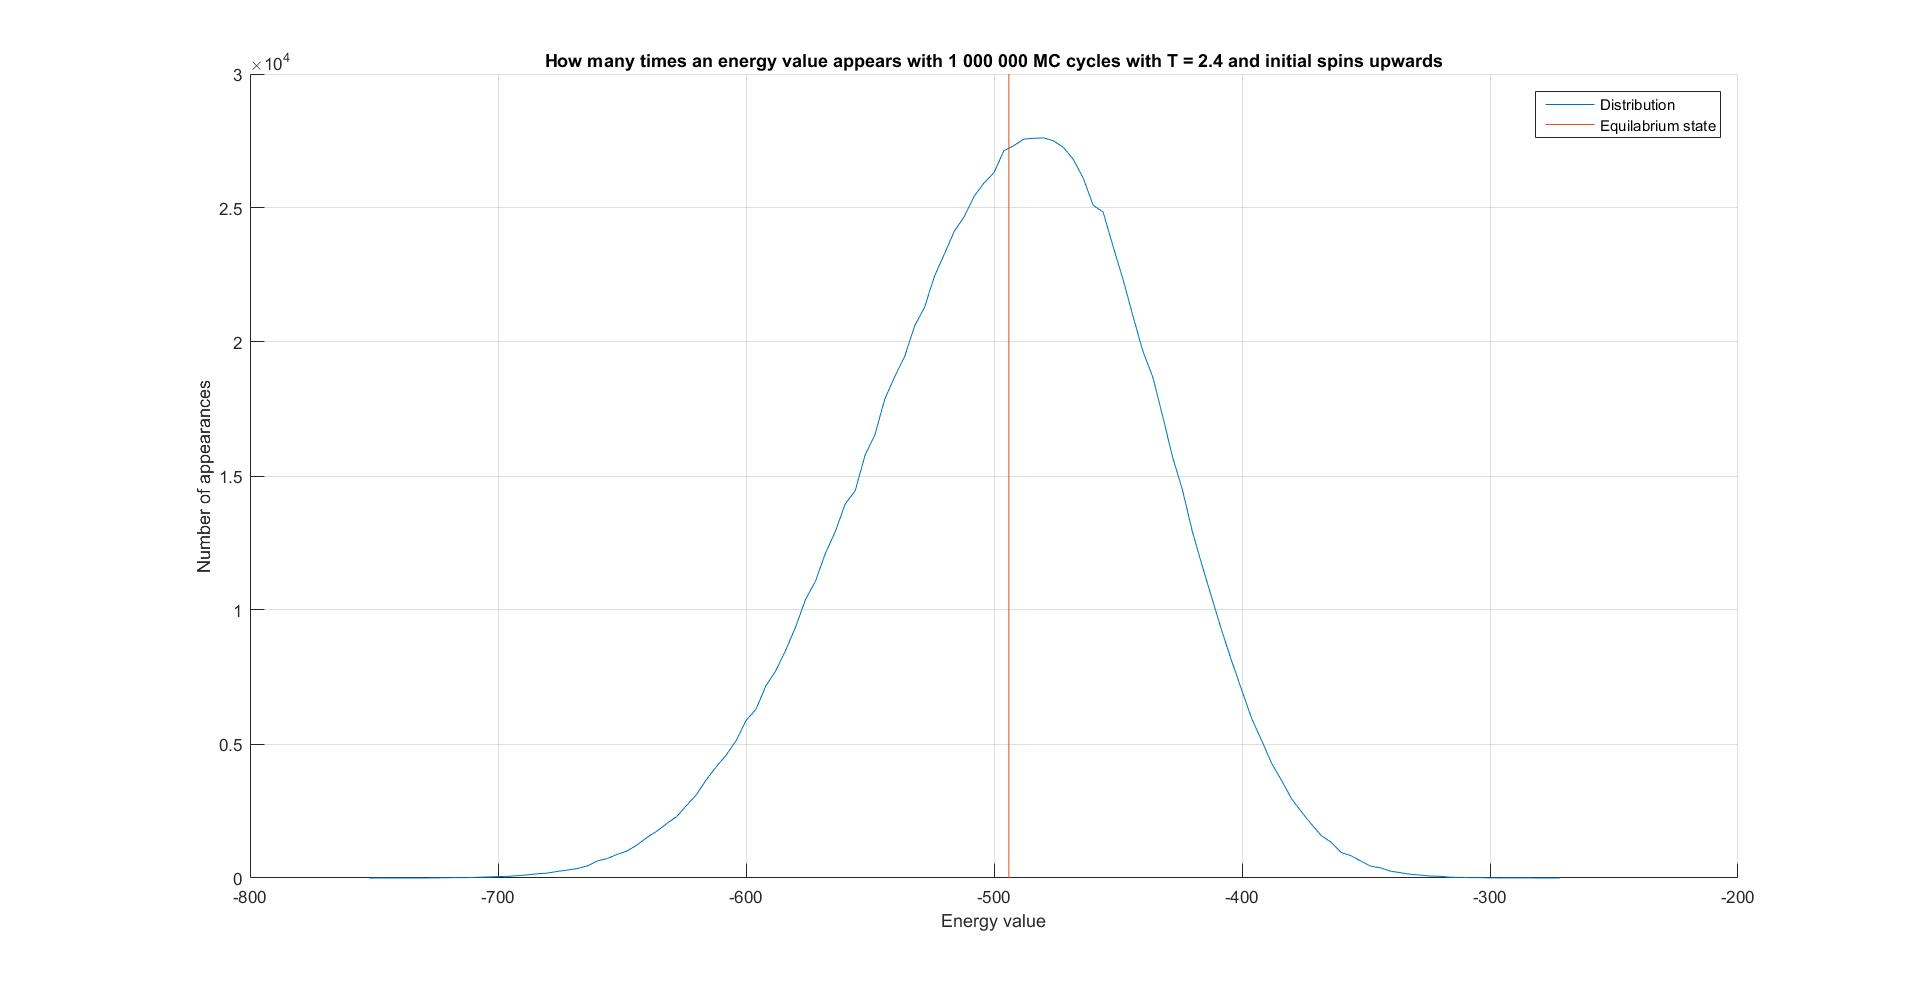
\includegraphics[width=0.7\textwidth]{energyappearanceT24upspin}
}
\caption{Number of appearances per energy value for a random initial matrix and with initial spin upwards when T = 2.4}
\label{fig:energyappearance}
\end{figure}

\noindent With a randomly generated initial matrix, the variance computed in c++ becomes 3226.62. The calculated variance from the energy becomes 3226.9 for $10^6$ MC cycles (calculated in MatLab script "howmanytimes.m"). This gives great confidence in the variance. For an initial matrix where all the spins point upwards, the calculated variance in c++ becomes 3236.05. The variance calculated from energy values in MatLab becomes 3236.3, again showing the stability of the variance for $10^6$ MC cycles. With fewer MC cycles, the two variances calculated does not correlate. Variances for other temperatures are shown in the table below:
\begin{table}[H]
\caption{Variance for different temperatures} \label{tab:table4}
\centerline{
\begin{tabular}{|c|c|}
\hline
  Temperature & Variance\\
\hline
  T=1.0 & 10.1022\\
\hline
  T=1.25 & 52.89957\\
\hline
  T=1.50 & 181.264\\
\hline
  T=1.75 & 478.217\\
\hline
  T=2.0 & 1157.11\\
\hline 
  T=2.25 & 3145.31\\
\hline 
  T= 2.50 & 2479.27 \\
\hline 
  T=2.75 & 1690.68\\
\hline
  T=3.0 & 1445.93\\
\hline
\end{tabular}
}
\end{table}

\noindent One can observe from \figref{energyappearance} that the curves are slightly skewed towards the higher energy values. The curve is bell shaped and somewhat centred around the equilibrium state for the lattice at temperature $T = 2.4$ which is $-497$ and $-493$. 
\\
The run time for higher order lattices increased as the lattice size increased. The run times are shown in the table below:

\begin{table}[H]
\caption{Run time for different lattice sizes with $10^6$} \label{tab:table5}
\centerline{
\begin{tabular}{|c|c|}
\hline
  Lattice size & Run time in seconds\\
\hline
  20x20 & ???\\
\hline
  40x40 & ???\\
\hline
  60x60 & 3996.57\\
\hline
  80x80 & 7081.15\\
\hline
  100x100 & 18630.9\\
\hline 
  120x120 & ???\\
\hline
\end{tabular}
}
\end{table}

\begin{figure}[H]
\centerline{
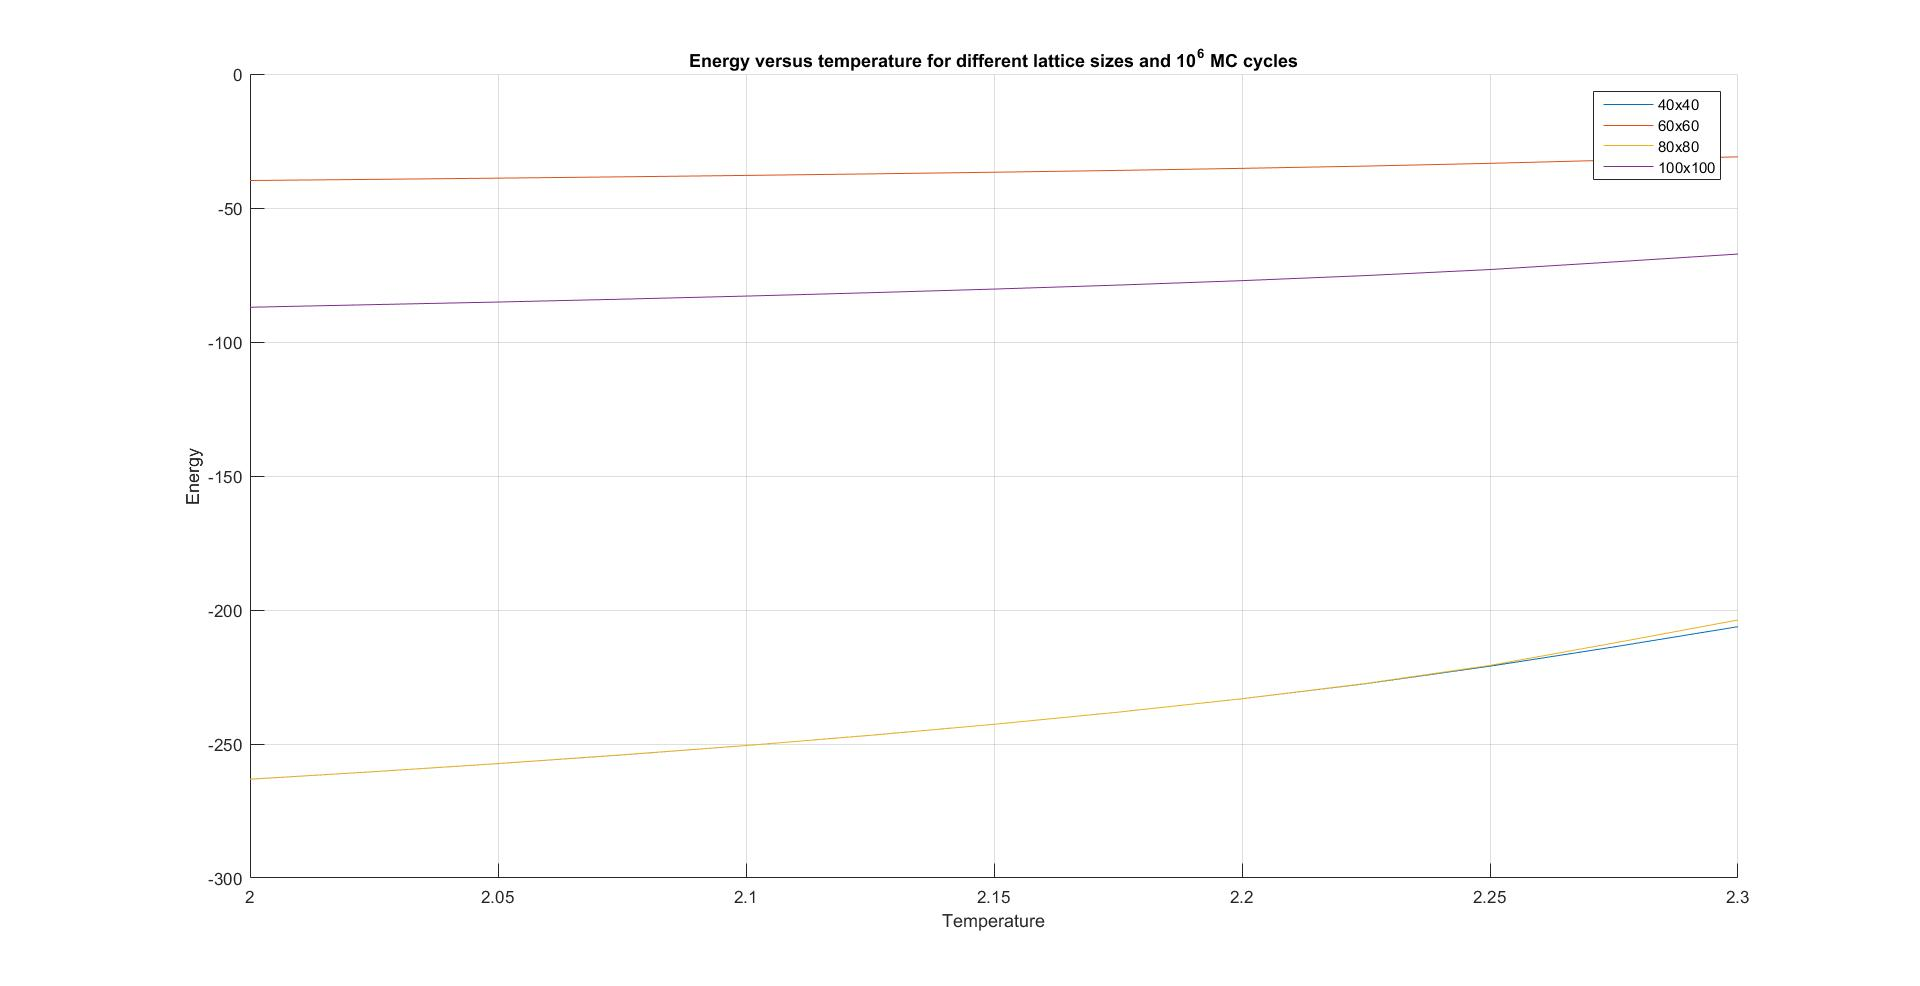
\includegraphics[width=0.7\textwidth]{energyVSt}
}
\caption{Mean energy versus temperature for $10^6$ Monte Carlo cycles for single lattice objects}
\label{fig:energyVSt}
\end{figure}

\begin{figure}[H]
\centerline{
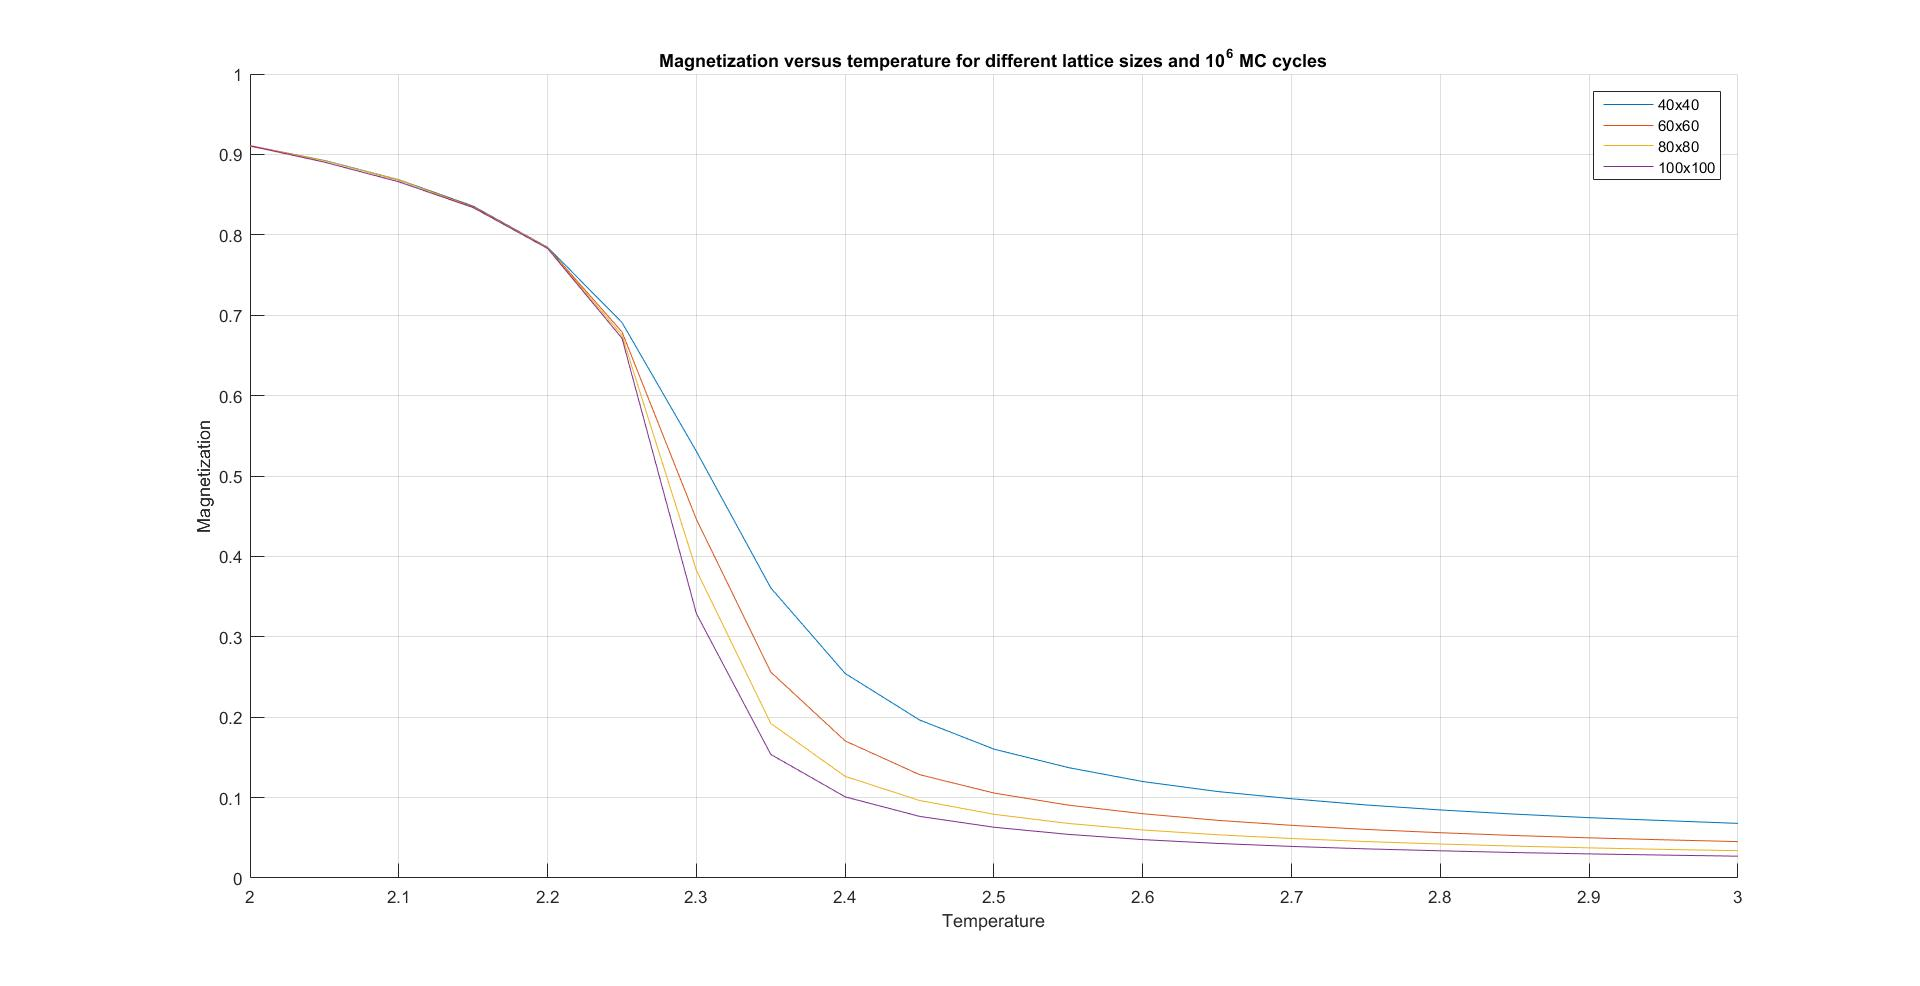
\includegraphics[width=0.7\textwidth]{magnetizationVSt}
}
\caption{Mean magnetization versus temperature for $10^6$ Monte Carlo cycles for single lattice objects}
\label{fig:magVSt}
\end{figure}

\begin{figure}[H]
\centerline{
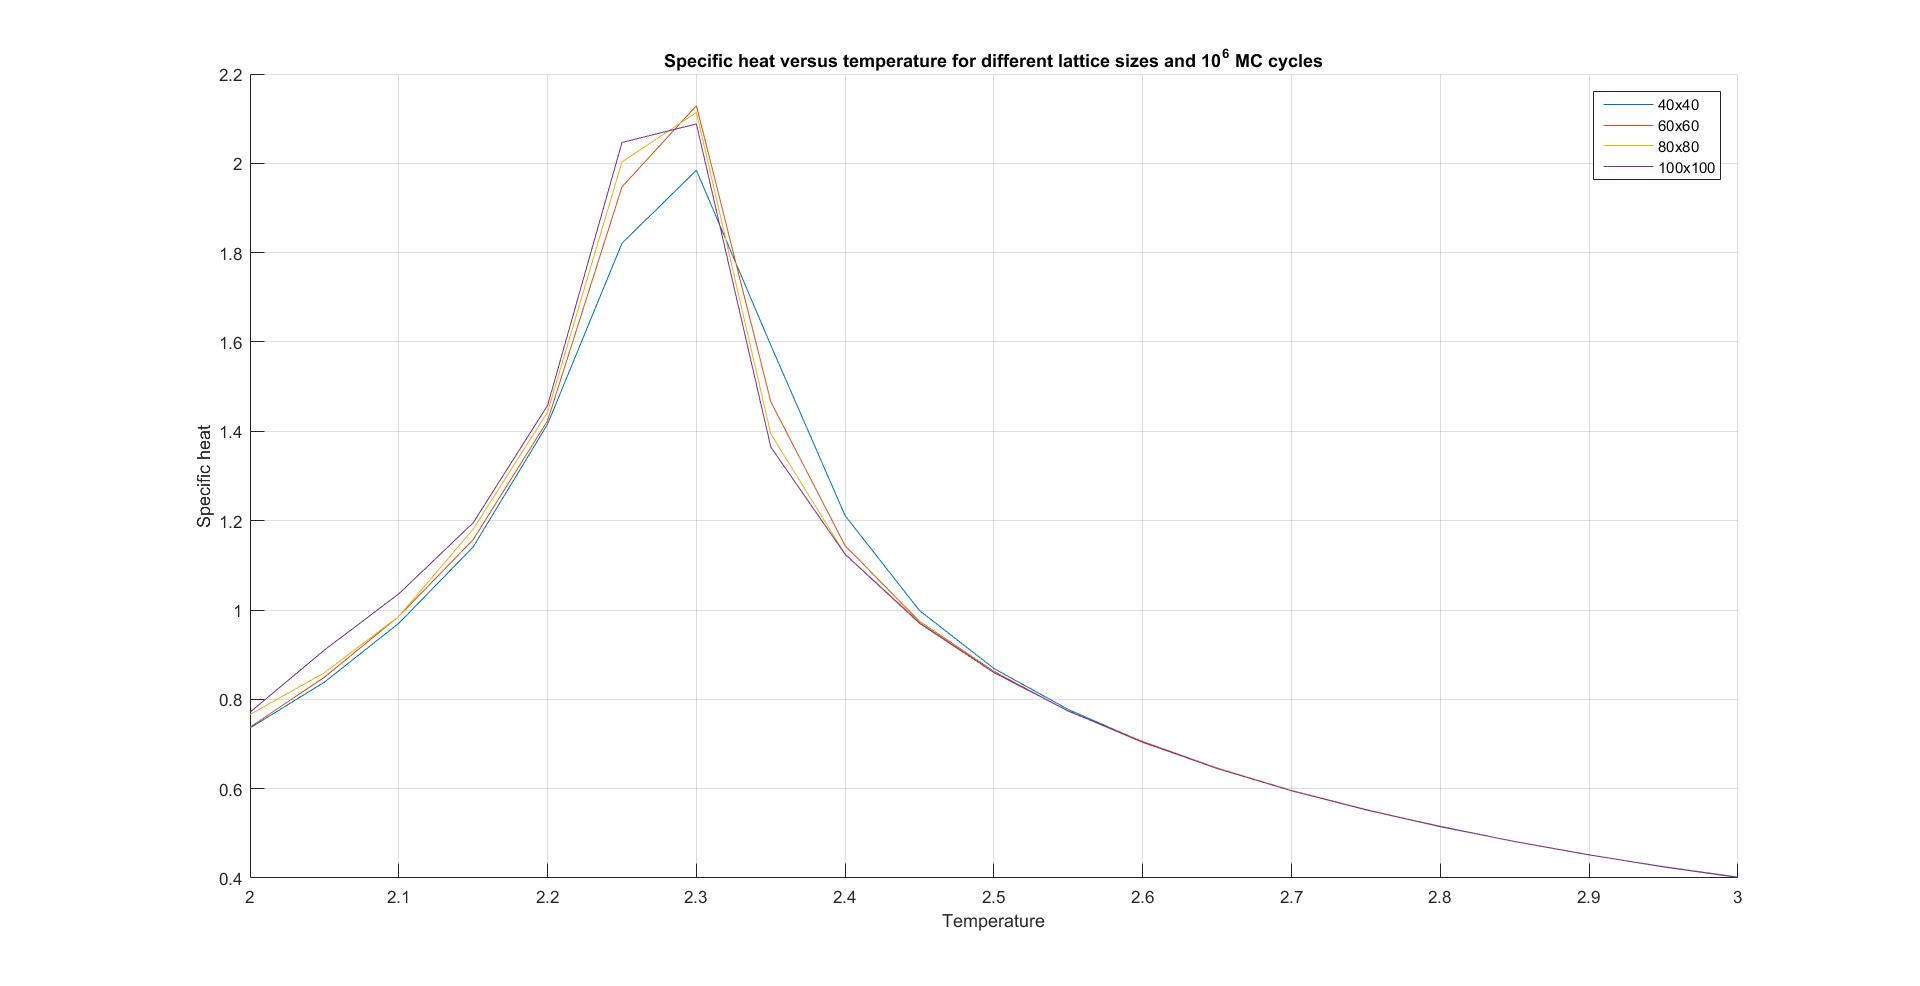
\includegraphics[width=0.7\textwidth]{heatVSt}
}
\caption{Specific heat versus temperature for $10^6$ Monte Carlo cycles for single lattice objects}
\label{fig:heatVSt}
\end{figure}

\begin{figure}[H]
\centerline{
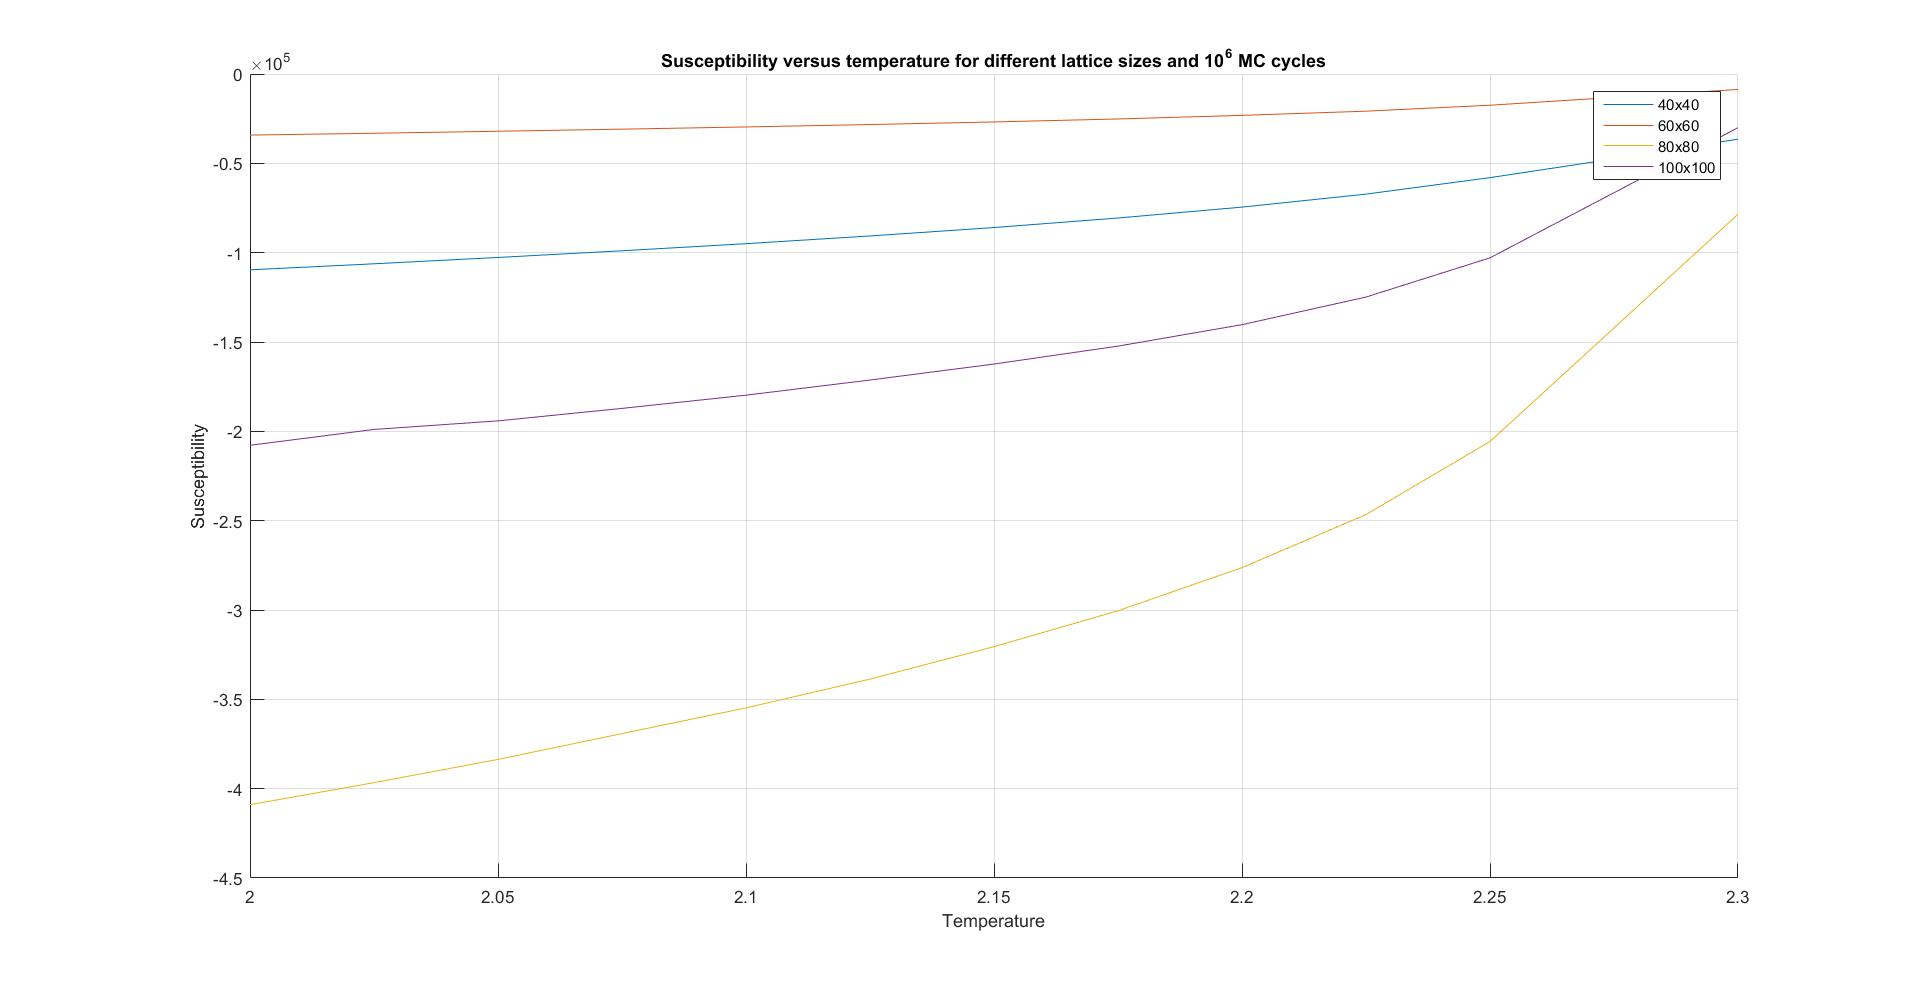
\includegraphics[width=0.7\textwidth]{susceptibilityVSt}
}
\caption{Susceptibility versus temperature for $10^6$ Monte Carlo cycles for single lattice objects}
\label{fig:susVSt}
\end{figure}

\noindent In the above figures, the respective values are representing an individual object in the lattice, not the entirety of the lattice. This was done because the graphs gave a clearer picture of what was going on. One can observe from \figref{energyVSt} that 

\newpage

\begin{center}
{\LARGE\bf Discussion}
\end{center}

\noindent Comparing Table \ref{tab:table2} and to \figref{energy1T} and \figref{energy24T} one can observe that the graph approaches the equilibrium value stated in the table. This is very clear for $T = 1.0$, but when $T = 2.4$, the energy seems to be oscillate which is natural due to the increased temperature in the system (kilde). Even though the value slightly oscillates after reaching equilibrium, the energy is still said to have reached equilibrium as stated in Table \ref{tab:table2} after a certain number of Monte Carlo cycles.
\\
The mean magnetization plotted on \figref{mag24T} show the magnetization without the absolute value and tells us that the magnetization actually jumps from positive to negative magnetization, and vice versa, rather quickly and frequent after reaching equilibrium. The reason for this is because the energy values are equal for symmetric magnetization values around the equilibrium state (kilde). This makes it easy for the magnetization to make these kind of leaps. Looking at \figref{absmag1T} and \figref{absmag24T}, the absolute value of the magnetization, we lose the above understanding, but we get the correct values, as calculated in c++, for the equilibrium state.
\\
This statement is only true when $T = 2.4$, because one can observe on \figref{mag1T} that when $T = 1.0$ the magnetization does not fluctuate for positive and negative values. It seems as the magnetization reaches it equilibrium state and then shortly jump to some negative value, then right back to the equilibrium value. The reason for this is because the temperature in the system is too low for the magnetization to make any great leaps (kilde). From the Boltzmann distribution we can see this mathematically:

$$
w_i = e^{-E_i/T}
$$

\noindent where $w_i$ is the probability, $E_i$ is the energy for and $T$ is the temperature. One can immediately see that when the temperature increase, the probability also increase for low energy values.

\noindent This means that the likelihood of flipping the orientation of the objects in the lattice should be higher for $T = 2.4$, since the probability of flipping should be higher than a random number. The magnetization and energy would then fluctuate more when $T = 2.4$ and this is observed on  \figref{energy1T},  \figref{energy24T}, \figref{absmag1T} and \figref{absmag24T}.
\\
Following this train of thought, one would expect the rate of acceptance to be greater for higher temperature values and this can be seen by comparing the y-axis on \figref{acceptancerandom} and \figref{acceptanceupspin}. This is confirmed on \figref{acceptancetemp} where the acceptance increases when the temperature increases. When the initial matrix is randomized, the results for low temperatures vary, due to the initial starting condition. This does not happen when the initial matrix only has upwards spin since the acceptance does not have to stabilize.
\\
Looking at \figref{energyappearance}, one clearly sees that both graphs are skewed towards higher energy values, when one may have expected the curve to center around it's equilibrium state. The largest area is to the left of the equilibrium, meaning most values is accepted here in the Metropolis algorithm. This makes sense because more values are accepted when the energy is lower according to the Boltzmann distribution, which can be observed on the graphs on \figref{energyappearance}.





\end{document}